% ******************************************************
% A Classic Thesis Style
% An Homage to The Elements of Typographic Style
%
% Copyright (C) 2018 André Miede and Ivo Pletikosić
% ******************************************************
\RequirePackage{silence}
    \WarningFilter{scrreprt}{Usage of this version of package `titlesec'}
    \WarningFilter{scrreprt}{Usage of package `tocloft' together}
    \WarningFilter{titlesec}{Non standard sectioning command}
\documentclass[
    twoside,
    openright,
    titlepage,
    numbers=noenddot,
    headinclude,
    footinclude,
    cleardoublepage=empty,
    abstract=on,
    BCOR=5mm,
    paper=a4,
    fontsize=11pt
]{scrreprt}

% ******************************************************
% Note: Make all your adjustments in here
% ******************************************************
\PassOptionsToPackage{utf8}{inputenc}
\usepackage{inputenc}

\PassOptionsToPackage{T1}{fontenc}
\usepackage{fontenc}


% ********************************************************************
% 1. Configure classicthesis for your needs here, e.g., remove "drafting" below
% in order to deactivate the time-stamp on the pages
% (see ClassicThesis.pdf for more information):
% ********************************************************************
\PassOptionsToPackage{
    drafting=true,    % print version information on the bottom of the pages
    tocaligned=false, % the left column of the toc will be aligned (no indentation)
    dottedtoc=false,  % page numbers in ToC flushed right
    eulerchapternumbers=true, % use AMS Euler for chapter font (otherwise Palatino)
    linedheaders=false,       % chaper headers will have line above and beneath
    floatperchapter=true,     % numbering per chapter for all floats (i.e., Figure 1.1)
    eulermath=false,  % use awesome Euler fonts for mathematical formulae (only with pdfLaTeX)
    beramono=true,    % toggle a nice monospaced font (w/ bold)
    palatino=true,    % deactivate standard font for loading another one, see the last section at the end of this file for suggestions
    style=classicthesis % classicthesis, arsclassica
}{classicthesis}


% ********************************************************************
% 2. Personal data and user ad-hoc commands (insert your own data here)
% ********************************************************************
\newcommand{\myTitle}{Quantum Circuit Compilation From The Ground Up\xspace}
\newcommand{\mySubtitle}{\xspace}
\newcommand{\myDegree}{Master of Mathematics (MMath)\xspace}
\newcommand{\myName}{Nathaniel Stemen\xspace}
% \newcommand{\myProf}{Someone else TODO\xspace}
\newcommand{\mySupervisor}{Joel Wallman\xspace}
\newcommand{\myFaculty}{Faculty of Mathematics\xspace}
\newcommand{\myDepartment}{Department of Applied Mathematics\xspace}
\newcommand{\myUni}{University of Waterloo\xspace}
\newcommand{\myInst}{Institute for Quantum Computing\xspace}
\newcommand{\myLocation}{Seattle, WA\xspace}
\newcommand{\myTime}{April 2022\xspace}
\newcommand{\myTimeFrame}{September 2020---April 2022}
\newcommand{\myVersion}{\classicthesis}

% ********************************************************************
% Setup, finetuning, and useful commands
% ********************************************************************
\newcommand{\ie}{i.\,e.}
\newcommand{\Ie}{I.\,e.}
\newcommand{\eg}{e.\,g.}
\newcommand{\Eg}{E.\,g.}


% ********************************************************************
% 3. Loading some handy packages
% ********************************************************************

% ********************************************************************
% Packages with options that might require adjustments
% ********************************************************************
\PassOptionsToPackage{american}{babel}
\usepackage{babel}

\usepackage{csquotes}

\PassOptionsToPackage{
    style=alphabetic,
    maxnames=5,
    backref=true
}{biblatex}
\usepackage{biblatex}

\PassOptionsToPackage{fleqn}{amsmath} % float equations towards left side
\usepackage{amsmath}
\newtheorem{theorem}{Theorem}[section]
\newtheorem{definition}[theorem]{Definition}
\newtheorem{example}[theorem]{Example}
\newtheorem{question}[theorem]{Question}

\usepackage{physics}
\usepackage{mathtools}
\usepackage{stmaryrd}
\DeclarePairedDelimiter\dbrackets{\llbracket}{\rrbracket}

% ********************************************************************
% General useful packages
% ********************************************************************
\usepackage{graphicx}
\usepackage{scrhack} % fix warnings when using KOMA with listings package
\usepackage{xspace} % to get the spacing after macros right
\PassOptionsToPackage{printonlyused,smaller}{acronym}
\usepackage{acronym} % TODO change to acro package


% ********************************************************************
% 4. Setup floats: tables, (sub)figures, and captions
% ********************************************************************
\usepackage{tabularx} % better tables: TODO change to booktabs
\setlength{\extrarowheight}{3pt} % increase table row height
\newcommand{\tableheadline}[1]{\multicolumn{1}{l}{\spacedlowsmallcaps{#1}}}
\newcommand{\myfloatalign}{\centering} % to be used with each float for alignment
\usepackage{subfig}


% ********************************************************************
% 5. Setup code listings
% ********************************************************************
\usepackage{listings}
%\lstset{emph={trueIndex,root},emphstyle=\color{BlueViolet}}%\underbar} % for special keywords
\lstset{language=[LaTeX]Tex,%C++,
    morekeywords={PassOptionsToPackage,selectlanguage},
    keywordstyle=\color{RoyalBlue},%\bfseries,
    basicstyle=\small\ttfamily,
    %identifierstyle=\color{NavyBlue},
    commentstyle=\color{Green}\ttfamily,
    stringstyle=\rmfamily,
    numbers=none,%left,%
    numberstyle=\scriptsize,%\tiny
    stepnumber=5,
    numbersep=8pt,
    showstringspaces=false,
    breaklines=true,
    %frameround=ftff,
    %frame=single,
    belowcaptionskip=.75\baselineskip
    %frame=L
}


% ********************************************************************
% 6. Last calls before the bar closes
% ********************************************************************
\usepackage{classicthesis}


% ********************************************************************
% Fine-tune hyperreferences (hyperref should be called last)
% ********************************************************************
\hypersetup{%
    %draft, % hyperref's draft mode, for printing see below
    colorlinks=true, linktocpage=true, pdfstartpage=3, pdfstartview=FitV,
    % uncomment the following line if you want to have black links (e.g., for printing)
    %colorlinks=false, linktocpage=false, pdfstartpage=3, pdfstartview=FitV, pdfborder={0 0 0},%
    breaklinks=true, pageanchor=true,
    pdfpagemode=UseNone,
    % pdfpagemode=UseOutlines,%
    plainpages=false, bookmarksnumbered, bookmarksopen=true, bookmarksopenlevel=1,%
    hypertexnames=true, pdfhighlight=/O,%nesting=true,%frenchlinks,%
    urlcolor=CTurl, linkcolor=CTlink, citecolor=CTcitation, %pagecolor=RoyalBlue,%
    %urlcolor=Black, linkcolor=Black, citecolor=Black, %pagecolor=Black,%
    pdftitle={\myTitle},
    pdfauthor={\textcopyright\ \myName, \myUni},
    pdfsubject={},
    pdfkeywords={},
    pdfcreator={pdfLaTeX},
    pdfproducer={LaTeX with hyperref and classicthesis}
}


% ********************************************************************
% Setup autoreferences (hyperref and babel)
% ********************************************************************
% There are some issues regarding autorefnames
% http://www.tex.ac.uk/cgi-bin/texfaq2html?label=latexwords
% you have to redefine the macros for the
% language you use, e.g., american, ngerman
% (as chosen when loading babel/AtBeginDocument)
% ********************************************************************
\makeatletter
\@ifpackageloaded{babel}%
{%
    \addto\extrasamerican{%
        \renewcommand*{\figureautorefname}{Figure}%
        \renewcommand*{\tableautorefname}{Table}%
        \renewcommand*{\partautorefname}{Part}%
        \renewcommand*{\chapterautorefname}{Chapter}%
        \renewcommand*{\sectionautorefname}{Section}%
        \renewcommand*{\subsectionautorefname}{Section}%
        \renewcommand*{\subsubsectionautorefname}{Section}%
    }%
    % Fix to getting autorefs for subfigures right (thanks to Belinda Vogt for changing the definition)
    \providecommand{\subfigureautorefname}{\figureautorefname}%
}{\relax}
\makeatother


\newcommand{\N}{\mathbb{N}}
% \newcommand{\Z}{\mathbb{Z}}
% \newcommand{\Q}{\mathbb{Q}}
\newcommand{\R}{\mathbb{R}}
\newcommand{\C}{\mathbb{C}}
% \renewcommand{\H}{\mathbb{H}}
\newcommand{\F}{\mathbb{F}}
\newcommand{\1}{\mathbb{1}}
\newcommand{\iu}{\mkern1mu\mathrm{i}\mkern1mu}
% \newcommand{\ju}{\mkern1mu\mathrm{j}\mkern1mu}
% \newcommand{\ku}{\mkern1mu\mathrm{k}\mkern1mu}
\newcommand{\e}{\mathrm{e}}
\newcommand{\mats}[2]{\mathcal{M}_{#1}(#2)}
% \newcommand{\GL}[2]{\mathsf{GL}(#1;\, #2)}
% \newcommand{\GLV}[1]{\mathsf{GL}(#1)}
% \newcommand{\SL}[2]{\mathsf{SL}(#1;\, #2)}
\newcommand{\U}[1]{\mathsf{U} (#1)}
\newcommand{\PU}[1]{\mathsf{PU} (#1)}
\newcommand{\SU}[1]{\mathsf{SU} (#1)}
% \renewcommand{\O}[1]{\mathsf{O}(#1)}
% \newcommand{\SO}[1]{\mathsf{SO}(#1)}
% \newcommand{\Sp}[1]{\mathsf{Sp}(#1)}
% \newcommand{\Spf}[2]{\mathsf{Sp}(#1;\, #2)}

\newcommand{\CNOT}{\ensuremath{\mathsf{CNOT}}}
\newcommand{\CCNOT}{\ensuremath{\mathsf{CCNOT}}}
\newcommand{\SWAP}{\ensuremath{\mathsf{SWAP}}}
\newcommand{\controlled}[1]{\ensuremath{\mathsf{Controlled}\text{-}#1}}

% \newcommand{\gl}[2]{\mathsf{gl}(#1;\, #2)}
% \newcommand{\glV}[1]{\mathsf{gl}(#1)}
% \newcommand{\slie}[2]{\mathsf{sl}(#1;\, #2)}
% \renewcommand{\u}[1]{\mathsf{u}(#1)}
% \newcommand{\su}[1]{\mathsf{su}(#1)}
% \newcommand{\so}[1]{\mathsf{so}(#1)}

% \newcommand{\mfr}[1]{\mathfrak{#1}}
\newcommand{\conj}[1]{\overline{#1}}
% \newcommand{\laplace}{\triangle}
\newcommand{\free}[1]{\expval{#1}}

\newcommand{\defeq}{\coloneqq}%\stackrel{\text{\tiny def}}{=}}
\newcommand{\eqdef}{\eqqcolon}%\stackrel{\text{\tiny def}}{=}}
\DeclareMathOperator{\vspan}{span}
\DeclareMathOperator{\vectorize}{vec}
\DeclareMathOperator{\arity}{arity}
\DeclareMathOperator{\qubits}{qubits}
% \DeclareMathOperator{\Ad}{Ad}
% \DeclareMathOperator{\ad}{ad}
\DeclareMathOperator{\id}{id}
% \DeclareMathOperator{\im}{im}
\DeclareMathOperator{\Hom}{Hom}
\DeclareMathOperator{\End}{End}
\DeclareMathOperator{\Aut}{Aut}
% \DeclareMathOperator{\Sym}{Sym}
% \DeclareMathOperator{\Lie}{Lie}
% \DeclareMathOperator{\column}{col}
% \DeclareMathOperator{\spectrum}{spectrum}
% \DeclareMathOperator{\diag}{diag}
\DeclareMathOperator*{\argmin}{arg\,min}
% \newcommand{\col}[2]{\column(#1, #2)}
\DeclareMathOperator{\Fid}{F}


% Non math
\newcommand{\ie}{i.\,e.}
\newcommand{\Ie}{I.\,e.}
\newcommand{\eg}{e.\,g.}
\newcommand{\Eg}{E.\,g.}

\def\CPP{{C\nolinebreak[4]\raisebox{.15ex}{++}}}

\usepackage{tikz} % TODO is this needed
\usetikzlibrary{arrows,shadows,positioning,fit}
\usetikzlibrary{quantikz}

\usepackage[style=super, sort=use]{glossaries}
\newglossary*{symbols}{List of Symbols}
\makeglossaries

\usepackage{attrib}
\usepackage{enumitem}
\usepackage{qtree}
\usepackage{standalone}
\usepackage{wrapfig}
\usepackage{cleveref}

\newlist{requirements}{enumerate}{10}
\setlist[requirements]{label*=\arabic*.}
\crefname{requirementsi}{requirements}{requirements}
\Crefname{requirementsi}{Requirements}{Requirements}

\newtheorem{theorem}{Theorem}[section]
\newtheorem{definition}[theorem]{Definition}
\newtheorem{example}[theorem]{Example}
\newtheorem{question}[theorem]{Question}

% ******************************************************
% Bibliographies
% ******************************************************
\addbibresource{bib.bib}

% ******************************************************
% Hyphenation
% ******************************************************
%\hyphenation{put special hyphenation here}

% ******************************************************
% GO!GO!GO! MOVE IT!
% ******************************************************
\begin{document}
\frenchspacing
\raggedbottom
\selectlanguage{american}
\pagenumbering{roman}
\pagestyle{plain}
% ******************************************************
% Frontmatter
% ******************************************************
%*******************************************************
% Titlepage
%*******************************************************
\begin{titlepage}
    % \pdfbookmark[1]{\myTitle}{titlepage}
    % if you want the titlepage to be centered, uncomment and fine-tune the line below (KOMA classes environment)
    \begin{addmargin}[-1cm]{-3cm}
    \begin{center}
        \large

        \hfill

        \vfill

        \begingroup
            \color{CTtitle}\spacedallcaps{\myTitle} \\ \bigskip
        \endgroup

        \spacedlowsmallcaps{\myName}

        \vfill

        
\includegraphics[width=6cm]{img/uwlogo} \\ \medskip

        \myDegree \\
        \myDepartment \\
        \myUni \\ \bigskip

        \myTime\ -- \myVersion

        \vfill

    \end{center}
  \end{addmargin}
\end{titlepage}

\thispagestyle{empty}

\hfill

\vfill

\noindent\myName: \textit{\myTitle,} \myDegree,
\textcopyright\ \myTime

\bigskip

\noindent\spacedlowsmallcaps{Supervisors}: \\
\mySupervisor

\medskip

\noindent\spacedlowsmallcaps{Location}: \\
\myLocation (completed remotely during COVID-19)

\medskip

\noindent\spacedlowsmallcaps{Time Frame}: \\
\myTimeFrame

\cleardoublepage%*******************************************************
% Dedication
%*******************************************************
\thispagestyle{empty}
\phantomsection
\pdfbookmark[1]{Dedication}{Dedication}

\vspace*{3cm}

\begin{center}
    \emph{Ohana} means family. \\
    Family means nobody gets left behind, or forgotten. \\ \medskip
    --- Lilo \& Stitch
\end{center}

\medskip

\begin{center}
    Dedicated to the loving memory of Rudolf Miede. \\ \smallskip
    1939\,--\,2005
\end{center}

% \cleardoublepage\include{aux/foreword}
\cleardoublepage%*******************************************************
% Abstract
%*******************************************************
%\renewcommand{\abstractname}{Abstract}
\pdfbookmark[1]{Abstract}{Abstract}
% \addcontentsline{toc}{chapter}{\tocEntry{Abstract}}
\begingroup
\let\clearpage\relax
\let\cleardoublepage\relax
\let\cleardoublepage\relax

\chapter*{Abstract}
Short summary of the contents in English\dots a great guide by
Kent Beck how to write good abstracts can be found here:
\begin{center}
\url{https://plg.uwaterloo.ca/~migod/research/beckOOPSLA.html}
\end{center}

\vfill

\endgroup

\vfill

\cleardoublepage%*******************************************************
% Acknowledgments
%*******************************************************
\pdfbookmark[1]{Acknowledgments}{acknowledgments}

\begin{flushright}{\slshape %TODO
        We have seen that computer programming is an art, \\
        because it applies accumulated knowledge to the world, \\
        because it requires skill and ingenuity, and especially \\
        because it produces objects of beauty.} \\ \medskip
    % --- \defcitealias{knuth:1974}{Donald E. Knuth}\citetalias{knuth:1974} \citep{knuth:1974}
\end{flushright}



\bigskip

\begingroup
\let\clearpage\relax
\let\cleardoublepage\relax
\let\cleardoublepage\relax

\chapter*{Acknowledgments}

Many thanks are in place for the successful completion of this thesis.
First I would like to thank my academic advisor Joel Wallman for the guidance during my bumpy career as a graduate student.
In addition, thank you to the following professors to helping me complete my studies: John Watrous, Achim Kempf, Michael Waite, Brian Ingalls, and Michael Brannan.
Whether it was sharing details about your personal career, asking probing questions, or offering time and having supportive conversation despite not having to: thank you.

Thank you to Joel's research group for helping me deal with Joel's departure: Darian Mclaren, Anthony Chytros, Matthew Graydon, Stefanie Beale, Sam Ferracin, and Joshua Skanes-Norman.
I would also like to thank my many classmates without which remote classes would have been far less interesting and rewarding: Wilson Wu, Chelsea Komlo, Mohammad Ayyash, Nicholas Zutt, and Xiaoran Li.
A big thank you is also in order for Overleaf and in particular John Lees-Miller and Ryan Looney for allowing me to work part time and being extremely flexible with my hours.
It was great to supplement the measly graduate student salary.

Thank you Mom and Dad for letting me live in your house while we endured the brunt of the pandemic.
Thank you Diane for always having my back and being supportive throughout my graduate studies.
Thank you to my friends who were always open to discuss my struggles and triumphs: Kevin (both of you), Rafael, Ana, and Aimee.

\endgroup

\cleardoublepage% ******************************************************
% Table of Contents
% ******************************************************
\pagestyle{scrheadings}
%\phantomsection
\pdfbookmark[1]{\contentsname}{tableofcontents}
\setcounter{tocdepth}{2} % <-- 2 includes up to subsections in the ToC
\setcounter{secnumdepth}{3} % <-- 3 numbers up to subsubsections
\manualmark
\markboth{\spacedlowsmallcaps{\contentsname}}{\spacedlowsmallcaps{\contentsname}}
\tableofcontents
\automark[section]{chapter}
\renewcommand{\chaptermark}[1]{\markboth{\spacedlowsmallcaps{#1}}{\spacedlowsmallcaps{#1}}}
\renewcommand{\sectionmark}[1]{\markright{\textsc{\thesection}\enspace\spacedlowsmallcaps{#1}}}
% ******************************************************
% List of Figures and of the Tables
% ******************************************************
\clearpage
% \pagestyle{empty} % Uncomment this line if your lists should not have any headlines with section name and page number
\begingroup
\let\clearpage\relax
\let\cleardoublepage\relax
% ******************************************************
% List of Figures
% ******************************************************
%\phantomsection
%\addcontentsline{toc}{chapter}{\listfigurename}
\pdfbookmark[1]{\listfigurename}{lof}
\listoffigures

\vspace{8ex}

% ******************************************************
% List of Tables
% ******************************************************
%\phantomsection
%\addcontentsline{toc}{chapter}{\listtablename}
\pdfbookmark[1]{\listtablename}{lot}
\listoftables

\vspace{8ex}
% \newpage

% ******************************************************
% List of Listings
% ******************************************************
%\phantomsection
%\addcontentsline{toc}{chapter}{\lstlistlistingname}
\pdfbookmark[1]{\lstlistlistingname}{lol}
\lstlistoflistings

\vspace{8ex}

% ******************************************************
% Acronyms
% ******************************************************
%\phantomsection
\pdfbookmark[1]{Acronyms}{acronyms}
\markboth{\spacedlowsmallcaps{Acronyms}}{\spacedlowsmallcaps{Acronyms}}
\chapter*{Acronyms}
\begin{acronym}[UMLX]
    \acro{CPU}{Central Processing Unit}
    \acro{IR}{Intermediate Representation}
    \acro{MLIR}{Multi-Level Intermediate Representation}
    \acro{NISQ}{Noisy Intermediate-Scale Quantum}
    \acro{NIST}{National Institute of Standards and Technology}
\end{acronym}

\vspace{3ex}

% ******************************************************
% Symbols/Notation
% ******************************************************
\pdfbookmark[1]{List of Symbols}{symbols}
\newglossaryentry{un}{
    type=symbols,
    name={\ensuremath{\U{n}}},
    description={Group of Unitary operators or matrices of dimension $n\times n$}
}
\printglossaries

\endgroup

% ******************************************************
% Main matter
% ******************************************************
\cleardoublepage
\pagestyle{scrheadings}
\pagenumbering{arabic}
%\setcounter{page}{90}
% use \cleardoublepage here to avoid problems with pdfbookmark

\cleardoublepage

\ctparttext{
    To begin this document we will introduce the notion of a compiler and show the foundational role it plays in our modern computing infrastructure.
    We will cover the main ideas from compilers that are useful for our quest to understand quantum circuit compilers in~\cref{part:backend}.
    We will then switch gears to cover the basics of quantum computation needed to understand the quantum part of our story.
}
\part{Front End}\label{part:frontend}
%************************************************
\chapter{All Things Classical}\label{chap:compilers}
%************************************************

In this chapter we will give a very brief overview of the components of classical computers that will be helpful to further discussions of quantum circuit compilation.
A key component to quantum circuit compilation is the word ``compilation'' whose origins (in computing) date to the early 1950's when electronic digital computers were in their early stages.
Understanding the historical development of compilation and its techniques will provide ideas and tools necessary to solve the new task of quantum circuit compilation.

This chapter is meant to provide the reader with the basics of some computing terminology and ideas.
It is by no means a complete introduction to compilers, nor computer architecture.

\section{What can a computer do?}

If you're reading this, I'm sure you can imagine something your computer is capable of.
Maybe reading this document online, sending messages/email, browsing the internet, writing documents, etc.
These are very high-level operations our computer can perform, but under the hood much more primitive operations are taking place.
It is these primitive operations that we wish to understand, and will have many similarities with modern-day quantum hardware.

A simplified model of computer architecture, known as the von Neumann Architecture (\cref{fig:comparch}) shows what we now call a \ac{CPU} which is the workhorse of the computer.\footnote{At least in this \emph{very simplified} model.}

\begin{figure}[h]
    \centering
    \includestandalone[width=0.8\textwidth]{tikz/arch}
    \caption{von Neumann Architecture scheme}\label{fig:comparch}
\end{figure}

Since the \ac{CPU} is the computational component of the computer, what can \emph{it} do?
Modern \acp{CPU} are built on the \ac{ISA} which means that the \ac{CPU} has a finite set of operations or instructions that it can perform.
Every operation the computer can perform must be built up from these primitive instructions.
Some examples of what these primitive operations might be are:
\begin{itemize}
    \item put a value into memory;
    \item add two values in memory together and store the result in a new location;
    \item perform the bitwise negation on a value;
    \item compute the square root of a value.
\end{itemize}
One can then use these primitives to build up complex functionality that eventually implement the capabilities we know and love (and hate) computers for.
By choosing an \ac{ISA}, a \emph{complexity class} is created of all the problems that can be solved using a polynomial number of instructions.\footnote{Polynomial refers to the function which takes the \emph{size} of the problem input, and returns the number of steps (or time) required to solve the problem.}
In practice most \acp{ISA} implement the same complexity class which we denote by P and refers to decision problems solvable by a deterministic Turing machine in a polynomial amount of time. % TODO complexity
There are many \acp{ISA} one can come up with that spawn different complexity classes, of which the ones we expect some familiarity with are P and NP on the classical side, and BQP on the quantum side.
For more details on complexity classes consult~\cite{complexity} and~\cite[Chapter 3]{nielsenchuang}.

The \ac{ISA} architecture style has seen major success, but it suffers from the drawback of requiring the programmer to work at the very low-level of machine instructions.
To work at a higher level of abstraction, and hence to have a higher-level of productivity, computer scientists and programmers created new languages which were easier to read, write, and reason about.
This necessitated new languages to be ``translated'' into the instruction set after the code was written.
The software responsible for translating these higher level ideas into a machines instruction set are known as \textbf{compilers}.

\section{Compilers}

While compilers have their origins in the aforementioned translation of higher-level code into lower-level code, they have grown considerably to perform many more tasks.
Before we dive into all of the capabilities of modern compilers, let's take a step back and recall what the word compile means.

Merriam-Webster~\cite{compiledef} defines the word \emph{compile} to mean
\begin{quote}
    to compose out of materials from other documents.
\end{quote}
In the context of programming language compilers,  ``other documents'' might mean the code itself, as well as configuration files and environment variables.
With these materials the lower level machine code is then composed.
This definition is reflected in~\citetitle{dragonbook}\footnote{Colloquially known as ``The Dragon Book'' because of the cover, and likely the most famous book on (classical) compilers. This is also where the logo of the LLVM project originates from which we will discuss in~\cref{sec:llvm}.}\graffito{
    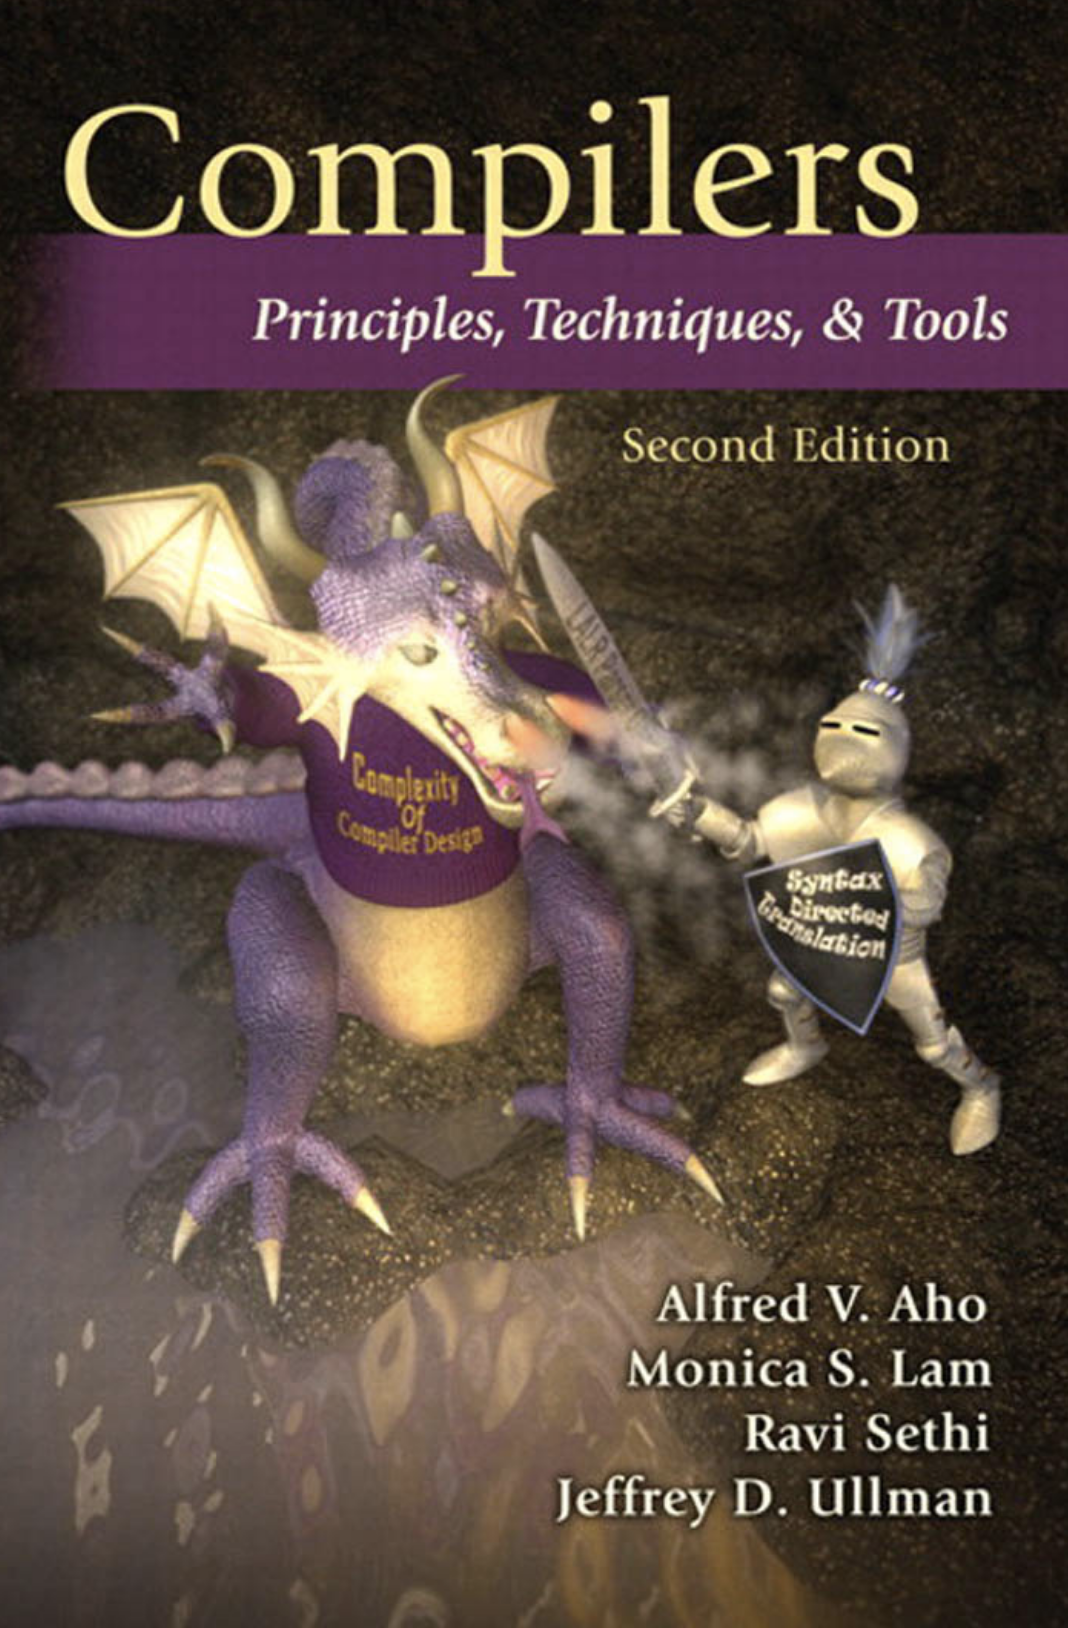
\includegraphics[width=\marginparwidth]{img/dragonbook.png}
    \emph{The Dragon Book}
    
\includegraphics[width=\marginparwidth]{img/llvmlogo.png}
    \emph{LLVM Logo}
}~\cite{dragonbook} where the authors introduce compilers through the process of transforming software.
\begin{quotation}
    [B]efore a program can be run, it first must be translated into a form in which it can be executed by a computer.

    The software systems that do this translation are called \emph{compilers}.
\end{quotation}
Hence we can view compilers as a function taking software written at one level of abstraction and bringing it down to a lower level that a computer's \ac{CPU} can understand.
\begin{figure}[ht]
    \centering
    \includestandalone[width=0.8\textwidth]{tikz/compiler}
    \caption{Action of Compiler}\label{fig:compiler}
\end{figure}

The term compiler was first used in the context computers by Grace Hopper in the early 1950's while working on a system that could translate symbolic mathematics into a machine language.
Initially Hopper's new idea was met with resistance as it was thought to be unrealistic.
\begin{quotation}
    I had a running compiler, and nobody would touch it because, they carefully told me, computers could only do arithmetic; they could not do programs.
    It was a selling job to get people to try it.
    I think with any new idea, because people are allergic to change, you have to get out and sell the idea.
    \attrib{Grace Hopper~\cite{hopperquote}}
\end{quotation}
In the end she succeeded in selling the idea and compilers have become a ubiquitous piece of modern computing infrastructure.
While Hopper's compiler focused solely on code translation, a modern compiler might perform all of line reconstruction, preprocessing, lexical analysis, syntax analysis, semantic analysis, conversion to an \ac{IR}, optimization (and there are many different types!), and finally code generation.
Thankfully we will not need to understand \emph{all} of these parts in full, but rather will focus on \aclp{IR}, optimizations, and code generation.

\subsection{Compilation Phases}\label{sec:comp-phases}

As alluded to in the previous section, a compiler has many different responsibilities.
Each responsibility is broken into a separate component so that it can be understood on its own.
A schematic for this can be seen in~\cref{fig:compilerphases} for the main steps that we will be concerned with in this document.
\begin{wrapfigure}[24]{i}{0.25\textwidth}% TODO tweak lineheight
    \centering
    \includestandalone[width=0.23\textwidth]{tikz/phases}
    \caption{Compiler Phases}\label{fig:compilerphases} % TODO can we fix this caption?
\end{wrapfigure}

\paragraph{Syntax Analyzer}
This phase is for ensuring the code is syntactically well formed (that is, that it abides by the specification of the language).
If one is writing code in a binary alphabet with characters \texttt{0} and \texttt{1}, then the ``program'' \texttt{00011} is syntactically valid, while \texttt{1102} is not because a \texttt{2} appears in the code.
Many compilers transform the code into a syntax tree to complete the verification.

\paragraph{Semantic Analyzer}
Now that the code is syntactically valid, we can ensure it has meaning.
This phase usually consists of type checking and scope validation (ensuring the code does not access variables outside of scope).
In many compiled languages the operation \texttt{'hello' * 5} would pass syntax analysis, but fail semantic analysis because a string multiplied by an integer is not a valid operation.\footnote{It is completely valid in other languages like Python, but Python is not a compiled language.}

\paragraph{Intermediate Code Generator}
The code is now ensured to be well formed and can begin preparation to execute on hardware.
Passing directly to the code generator is possible from here, but the end product will be slower as no optimizations will take place.
Instead, the existing code (or sometimes using the syntax tree created in the previous steps) will be transformed into an \acf{IR}.
This is a mid-level representation of the code in that it is typically thought of as somewhere between the high-level of abstraction of the programming language, and the low-level instruction set.

This is best seen with a simple example.
Suppose we have the following snippet to calculate the final location of a moving object after 5 seconds.
\begin{lstlisting}
    x_final = x_initial + velocity * 5
\end{lstlisting}
Upon transforming this code to an \ac{IR}, it takes on a more basic form.
\begin{lstlisting}
    t1 = inttofloat(5)
    t2 = velocity * t1
    t3 = x_initial + t2
    x_final = t3
\end{lstlisting}
The power here comes from the fact that the \acf{IR} can be language agnostic, and hence many languages can compile into the same \ac{IR}.
This design allows for the use of an optimizer for many languages.

\paragraph{Code Optimizer}
Once the code is in the \ac{IR}, the optimizer will attempt to ``improve'' it using many different methods.
Improve can mean many different things, but usually refers to runtime and memory use.
Optimizations that occur during this step are constant propagation, dead code elimination, removing unnecessary code from loops, and loop unrolling.
Optimizing the above example our code is still ``bulkier'' than originally written, but compressed in comparison to the original \ac{IR}-form.
\begin{lstlisting}
    t1 = velocity * 5.0
    x_final = x_initial + t1
\end{lstlisting}
Here we have skipped the call to \texttt{inttofloat} and instead immediately converted the integer \texttt{5} to the float \texttt{5.0}.
We have also combined two of the steps to reduce the number of temporary variables we have to create and store in memory.
As you can see the task of the optimizer is not only to try and speed up the code, but reduce its memory usage as well.
Some of the other problems the code optimizer must tackle are instruction selection, register allocation, and instruction scheduling all of which have analogs we will see in~\cref{chap:circuit-compilers}.

\paragraph{Code Generator}
Finally we have an optimized \ac{IR} and we can generate code for hardware.
This requires us to know which hardware it is we'd like to run our code on as each chip might have a different \ac{ISA}.
This is a very difficult step as many of the sub-problems that are required to be solved are themselves NP-complete such as register allocation~\cite{register-allocation-NP}. % TODO complexity
Further, generating mathematically optimal machine code has also been shown to be undecidable~\cite{dragonbook}!
Hence this step uses effective heuristics to solve the problem at hand in tractable amounts of time.
Typically this step is broken down into first optimizing the \ac{IR} for the hardware that has been chosen, followed by the actual code generation.
If this occurs the optimizer is typically referred to as a hardware-independent optimizer, and a later stage of optimizations is performed in a hardware-dependent optimizer.
We will see later that the distinct phases of optimization are of crucial importance when compiling quantum circuits.

Again following the above code example, upon code generation we may end with the following generic hardware instruction code.

\begin{minipage}{0.5\textwidth}
    \begin{lstlisting}
    LDF R2, velocity
    MULF R2, R2, #5.0
    LDF R1, x_initial
    ADDF R1, R1, R2
    STF x_final, R1
\end{lstlisting}
\end{minipage}
\begin{minipage}{0.5\textwidth}
    \centering
    \begin{tabular}{cc}
        Function      & Meaning         \\ \toprule
        \texttt{LDF}  & Load float      \\
        \texttt{MULF} & Multiply floats \\
        \texttt{ADDF} & Add floats      \\
        \texttt{STF}  & Store float
    \end{tabular}
    \captionof{table}{Machine Code}\label{fig:machcode}
\end{minipage}
Here anything beginning with \texttt{R} is a register.

The phases described here are often grouped into three larger categories.
The syntax and semantic analysis, as well as the generation of an \ac{IR} fall under the umbrella of ``front end'', the optimizer is the optimizer, and everything else that follows is the ``back end''.
The implications of this design is that an optimizer and backend can be paired with many different front ends as long as the front end can generate the optimizer's preferred \ac{IR} flavor.
\begin{figure}[ht]
    \centering
    \includestandalone[width=0.75\textwidth]{tikz/frontback}
    \caption{Compiler with many front and back ends}\label{fig:compends}
\end{figure}

\subsection{Optimizations}

Before moving on to some examples of compilers, its important to understand the separation of concerns in the two types of optimizations we've seen.
The main optimizer we see in~\cref{fig:compilerphases} as ``Code optimizer'' and again the ``Optimizer'' in~\cref{fig:compends} are typically where the majority of optimizations take place in classical compilers and are performed on an \ac{IR}.
One interesting class of examples are peephole optimizations~\cite{classical-peephole}.
These are optimizations that take advantage of small patterns found in code that can be simplified in some way.
Some examples are seen in~\cref{tab:peephole}.
\begin{table}[ht]
    \centering
    \begin{tabular}{p{.5\textwidth}l}
        Instruction                                                      & Optimized Instruction \\ \toprule
        Read value into a register, then immediately store it in memory. & Do nothing            \\
        $a \cdot x + b \cdot x$                                          & $(a + b) \cdot x$     \\
        $x - x$                                                          & $0$                   \\
        $(A^\intercal B^\intercal)^\intercal$                            & $BA$
    \end{tabular}
    \caption{Peephole Optimizations}\label{tab:peephole}
\end{table}
Other examples include dead code elimination, common subexpression elimination, and inlining.
The optimizations done here---usually to the ends of faster runtime and smaller memory use---are performed in the hopes that once the code is compiled into machine code it \emph{will} run faster.
The intuitive optimizations often remove duplication, but many other optimizations that are not so clear take advantage of the commonalities among \ac{CPU} design to produce code that will run faster on any \ac{CPU}.

With an optimized \ac{IR}, and a chosen backend, or hardware, the code can be modified to suit the instruction set, as well as other restrictions the hardware may place on computation.
For example, most \acp{CPU} have a small number of registers, and hence must use them wisely throughout the computation so as to use \emph{all} of them where possible, but not slow down computation by waiting for a register to be available.
Another example is instruction scheduling, where the compiler must figure out an optimal ordering to the computation, again to maximize the \acp{CPU} compute power while not causing bottlenecks.
There are many other examples of hardware-dependent optimizations, but as you might imagine, many require an intimate knowledge of the hardware's particular design.
All this transformation occurs while maintaining the same semantic meaning of the original program.

In summary the first hardware-independent optimization should be thought of as optimizing the implementation theoretically, and the hardware-dependent optimization as ensuring the optimized algorithm runs as fast as possible in its final implementation.
Many more examples of optimizations (both hardware-independent and hardware-dependent) can be found in~\cite[Chapter~8]{compiler-optimizations}.

\subsection{Examples}\label{sec:compiler-examples}

We've now seen what a compiler is and what we typically use it for.
A few examples are in order to help understand how compilers work in the real world, and just how varied they can be.

\begin{description}
    \item[clang:] Short for C Language, this is a compiler frontend for the C/\CPP{} languages. It takes in C/\CPP{} code and produces an LLVM \ac{IR} which we will learn about in~\cref{sec:llvm}. It then lets LLVM handle the rest of the compilation processing.
    \item[Latex:] While perhaps not very obvious, \LaTeX{} is indeed a compiler as it takes high-level formatting code, and produces a lower level representation of what the user wants to typeset. Usually that comes in the form of postscript which is another programming language that is read by printers (hardware) to produce the requested document. Postscript can also be read by PDF readers and browsers which then display content as the author desired (maybe).
    \item[TensorFlow:] TensorFlow is a library for machine learning that has drawn on the design principles of compilers in attempts to speed up and ensure the accuracy of models. Indeed it has a frontend where the user builds their model and compiles it into an \ac{IR} known as HLO \ac{IR} or High Level Operations. Typical optimizations then occur and again using the LLVM compiler infrastructure this code can be brought to many backends such as the browser, mobile, and specialized compute infrastructure (such as Google's \ac{TPU}). This is all before we talk about TensorFlow Quantum which allows for hybrid quantum-classical machine learning models~\cite{tensoflowquantum}.
\end{description}

\section{LLVM}\label{sec:llvm}

The LLVM\footnote{The project, while originally an acronym for Low Level Virtual Machine now goes solely by LLVM. The original name reflects the fact that the compiler targets low-level \ac{IR} code that runs on some theoretical (hence the term virtual) machine. Since the inception virtual machines have come to mean something different, hence the abandonment of the acronym.} project~\cite{llvm} is one of the largest open source compiler projects in existence and much of the compiler architecture we've discussed here come from its design.
The founder of the project Chris Lattner has characterized compilers succinctly in~\cite{lattnerquote} as
\begin{quote}
    the art of allowing humans to think at a level of abstraction that they want to think about.
\end{quote}

As an interesting historical note, once the \ac{ISA} scheme had become commonplace, chip designers began to implement more and more complex instructions on \acp{CPU} so that machine code became higher level.
At the same time, compilers became more popular, especially as their optimizations became more robust, and useful.
This led to a distinction between chip architectures known as \ac{CISC} and \ac{RISC}.
At the time of writing, \ac{CISC} processors are dominant in desktop computers, while \ac{RISC} processors emphasize efficiency and can be found in phones and many other portable computing hardware.
Some examples include Intel's x86 and x64 chips which are built in the \ac{CISC} style, while ARM is major designer of \ac{RISC} chips (including the most recent Apple Bionic A15 chip). % TODO add note about RISC V?
Today \acp{RISC} are sometimes referred to using the backronym ``Relegate Interesting Stuff to the Compiler''.

With the growth of LLVM, developers have pushed the compiler to extend its use to ``heterogeneous hardware''~\cite{mlir}, which already includes new types of computing hardware like \acp{TPU} and could in the future encompass a \ac{QPU}.
This is exciting not only because classical computer designers are beginning to consider quantum technologies as coprocessors, but because the monumental classical computing infrastructure can then be leveraged to aid in the solutions to quantum problems.
With the futurism, hype, and unknowns surrounding quantum technologies, it often seems that fundamentally new and ingenious ideas are needed to forward the field.
Projects such as the above show there are serious possibilities of recycling, or at the very least, learning from what has come before us.

%*****************************************
\chapter{Quantum Computation}\label{chap:quantum}
%*****************************************

In this chapter we will lay the groundwork for the necessary ideas from quantum computation.
We will not attempt to introduce quantum computation from the ground up, but instead introduce and emphasize the ideas needed for compiling quantum circuits.
The notation used here will mostly follow~\cite{watroustqi} and we recommend~\cite{nielsenchuang} for a more thorough introduction to the material.

\section{Historical Development}\label{sec:history}

One of the core tenets of quantum theory is that, at this scale, nature is reversible.
Hence, when physicist Charles H. Bennett began investigating reversible Turing machines~\cite{reversibleturing} we might say the field of quantum computing was \emph{just} getting started.
Since Turing machines are the mathematical and theoretical foundation for modern computers, it makes sense that a reversible Turing machine might lay the groundwork as the foundation for a computer that operators under quantum mechanical law.
More than 6 years later, Paul Benioff extended this work to describe a fully quantum mechanical version of a Turing machine in his paper \citetitle{quantumturing}~\cite{quantumturing}.

Once the theoretical foundation had been laid by Bennett and Benioff, Richard Feynman brought the idea mainstream when he proposed using these new computers to simulate quantum mechanics itself.
This idea was very attractive at the time (1981) since our classical computers were not powerful enough to simulate large quantum systems,\footnote{In fact, they still aren't!} and since Feynman was such a popular figure the idea finally took hold.
Feynman motivated the need for a new paradigm in computing as such.
\begin{quote}
    Nature isn't classical, dammit, and if you want to make a simulation of nature, you'd better make it quantum mechanical, and by golly it's a wonderful problem, because it doesn't look so easy.
    \attrib{Richard P. Feynman~\cite{feynmansimulator}}
\end{quote}

Even with one of the most famous physicists popularizing the idea, it took another 10 years to see the next major development which came when David Deutsch and Richard Jozsa gave an example of a problem that is solved exponentially faster on a quantum computer than a classical one~\cite{deutch-jozsa-algo}.
If there was any hesitancy from the academic community at this point about the theoretical usefulness of a quantum computer, this result showed real potential for the emerging technology.
More applications start rolling in with quantum teleportation~\cite{quantumteleportation} and famously Peter Shor's polynomial time algorithm to factor integers (and hence break many modern cryptosystems)~\cite{shor-encryption}.

The latter caught the eye of the US Government and within the year of Shor's publication the \ac{NIST} organized the first government funded conference on quantum computation.\footnote{It's likely this is when quantum computation was put on the radar of other US government agencies. In 2014 leaked documents showed the National Security Agency had begun a project dubbed ``Owning The Net'' whose purpose was to use a quantum computer to break internet cryptography and to ``gain access to and securely return high value target communications''. The status of the project---which also goes by the moniker ``Penetrating Hard Targets''---is unknown.}
With some of the theoretical groundwork and motivation laid through the 80's and 90's, the first experimental realization of a superconducting qubit was performed in~\citeyear{firstqubit} by Yasunobu Nakamura and Jaw-Shen Tsai~\cite{firstqubit}.
Fewer than 20 years passed
Hence it was fewer than 20 years after Feynman advocated the possibility of using quantum mechanics in a new type of computer that the idea was brought to fruition.

Since then ambitions have risen and technological progress has allowed for more and more qubits and quantum computers today have even been shown to complete tasks that classical ones cannot in any feasible amount of time.
In particular a team at China's Hefei National Laboratory used their 66-qubit computer\footnote{Affectionately named Zuchongzhi after Chinese mathematican Zu Chongzhi whose computation of $\pi$ was more accurate than any other for more than 800 years.} to complete a task in 4 hours that would take state of the art programs tens of thousands of years~\cite{zuchongzhi}.

In~\citeyear{nisq} John Preskill coined the term \ac{NISQ} as a characterization of quantum computers with a relatively small number of noisy qubits (50--100) with limited connectivity: \ie{} machines that have dominated the past decade, and will likely continue to for the next few years~\cite{nisq}.
The problem presented in this document is relevant to quantum computers past the \ac{NISQ}-era, but are especially important as we attempt to squeeze every ounce of computation out of them.

% TODO conclusion

\section{Quantum Computation}

In this section we will go over the basics of quantum computation.
Before continuing I would like to recommend~\cite{nielsenchuang} as well as \url{https://quantum.country} as great resources to learn the basics of quantum computing.

\subsection{Formalism}

A quantum bit, or \textbf{qubit} for short, is a vector $\ket{\psi}$ in 2-dimensional complex space $\C^2$ such that $\norm{\ket{\psi}} = 1$.
Often the following canonical basis is chosen and referred to as the computational basis.
\begin{align}
    \ket{0} \defeq \mqty[1 \\ 0] & & \ket{1} \defeq \mqty[0 \\ 1]
\end{align}
In this basis a qubit is represented as
\begin{equation}\label{eq:qubit}
    \ket{\psi} = \alpha\ket{0} + \beta\ket{1} = \mqty[\alpha \\ \beta]
\end{equation}
with the normalization condition that $\abs{\alpha}^2 + \abs{\beta}^2 = 1$.
In the case of \cref{eq:qubit} the state $\ket{\psi}$ is said to be in a \textbf{superposition} of state $\ket{0}$ and $\ket{1}$.

We often need to understand more complicated systems than just simple qubits, and to do so we use the \textbf{tensor product} to build up systems from subsystems.
\Eg{} if $\ket{\psi}\in\C^2$ and $\ket{\phi}\in\C^2$ represent two distinct physical qubits, we can represent the combined system as a single vector $\ket{\psi}\otimes \ket{\phi}$ in a larger complex Euclidean space $\C^2\otimes \C^2\cong \C^4$.
In many cases it is customary to drop the tensor product $\otimes$ symbol and write $\ket{\psi}\ket{\phi}$ or even $\ket{\psi \, \phi}$ when the underlying complex Euclidean spaces are understood.
In the computational basis we can expand this tensor product as
\begin{align}
    \ket{\psi}\otimes \ket{\phi} & = \qty(\alpha\ket{0} + \beta\ket{1})\otimes\qty(\gamma\ket{0} + \delta\ket{1})            \\
                                 & = \alpha\gamma\ket{00} + \alpha\delta\ket{01} + \beta\gamma\ket{10} + \beta\delta\ket{11}
\end{align}
where $\alpha, \beta, \gamma, \delta \in \C$.

With the objects of the theory defined, we must now understand the dynamics, or choreography of the theory.
As stated in~\cref{sec:history}, we take the theory of quantum mechanics to be reversible, and hence any operation we perform on a qubit $\ket{\psi}$ must be undo-able.
Thankfully linear algebra has just the tool to transform complex vectors in a reversible, and general way: unitary matrices!
\begin{definition}
    An $n\times n$ complex matrix $A$ is called \emph{unitary} if
    \begin{equation}\label{eq:unitary}
        AA^\dagger = A^\dagger A = \1
    \end{equation}
    where $^\dagger$ denotes the conjugate transpose.
    The collection of unitary matrices form a group known as the \emph{unitary group} and is denoted \gls{un}.
    This definition can also be stated simply using set builder notation;
    \begin{equation}
        \U{n} \defeq \qty{ A \in \mats{n}{\C} : AA^\dagger = \1 = A^\dagger A }
    \end{equation}
    where \gls{mats} is the set of all $n \times n$ complex matrices.
\end{definition}
Hence when we have a qubit $\ket{\psi}$ and perform some action on it, the new state is modeled by $\ket{\phi} = U\ket{\psi}$ where $U$ represents whatever action we performed.
The condition shown in~\cref{eq:unitary} is quite restrictive: where a general $n \times n$ matrix has $2n^2$ real degrees of freedom, an element of $\U{n}$ only has $n^2$.\footnote{This is to say $\dim_\R\U{n} = n^2$.}
In fact for a general element of $\U{2}$ we can decompose it into pieces that look much more familiar. % TODO transition from previous
\begin{example}\label{ex:u2decomp}
    Let $A$ be an arbitrary element of $\U{2}$.
    Then the following decomposition holds for $\alpha, \beta, \gamma, \delta \in \R$.
    \begin{equation}
        A = \e^{\iu\alpha}\mqty[\dmat[0]{\e^{-\iu \beta}, \e^{\iu \beta}}]\mqty[\cos\gamma & -\sin\gamma \\ \sin\gamma & \phantom{+}\cos\gamma]\mqty[\dmat[0]{\e^{-\iu \delta}, \e^{\iu \delta}}]
    \end{equation}
    As we can see the middle matrix is simply a 2-dimensional rotation matrix, and the other two are of a simple diagonal form.
    Lastly we have the global phase $\e^{\iu \alpha}$.
\end{example}

This is a particularly important example as the idea of decomposing unitary matrices into simpler pieces is something we will need heavily in circuit compilation tasks.
This decomposition also shows that each unitary in $\U{2}$ has a global phase ($\e^{\iu\alpha}$ in~\cref{ex:u2decomp}), which in quantum computation is often irrelevant as it is not experimentally measurable. % TODO cref wrong
For that reason we also often work in the following group where phases are removed.
\begin{definition}
    Define the \emph{projective unitary group} by taking the quotient of the unitary group $\U{n}$ by matrices of the form $\alpha \cdot \1$ where $\alpha$ is a unit length complex number.
    This is often written as follows, using a slight abuse of notation.
    \begin{equation}
        \gls{pun} \defeq \U{n} / \U{1}
    \end{equation}
\end{definition}
Elements of the projective unitary group are the smallest physically realizable set of operations in quantum computation, and hence they make sense as our starting point in the formalization process.

\subsection{Quantum Gates}

A \textbf{quantum gate} is a physically realizable, and unambigious mathematical transformation.
More formally, a quantum gate on $n$ qubits is an element $g \in \PU{2^n}$.
In this document we will mainly discuss quantum gates acting on 1 and 2 qubits as that is the capability of most modern hardware we will discuss in~\cref{chap:hardware}.
\Cref{tab:commongates} outlines some of the common gates we will encounter throughout this document, and their associated notations both mathematically, and diagrammatically.

\begin{table}[ht]
    \centering
    % \begin{noindent}
    \begin{tabular}{cccc}
        Name           & Notation & Circuit Diagram                                                                                 & Matrix                                                 \\ \toprule
        Pauli X        & $X$      & \begin{tikzcd} \qw & \gate{X} & \qw \end{tikzcd}                                                & $\smqty[0 & 1 \\ 1 & 0]$                               \\
        Pauli Z        & $Z$      & \begin{tikzcd} \qw & \gate{Z} & \qw \end{tikzcd}                                                & $\smqty[1 & \phantom{-}0 \\ 0 & -1]$                   \\
        Hadamard       & $H$      & \begin{tikzcd} \qw & \gate{H} & \qw \end{tikzcd}                                                & $\frac{1}{\sqrt{2}}\smqty[1 & \phantom{-}1 \\ 1 & -1]$ \\
        $\frac{\pi}{8}$-gate\tablefootnote{The name $\frac{\pi}{8}$-gate comes from the way the gate was first introduced in the literature, where it was written $T = \e^{\iu \pi / 8}\smqty[\e^{-\iu \pi / 8} & 0 \\ 0 & \e^{\iu \pi / 8}]$.}      & $T$      & \begin{tikzcd} \qw & \gate{T} & \qw \end{tikzcd}                                                & $\smqty[1 & 0 \\ 0 & \e^{\iu \pi/4}]$ \\
        Controlled Not & \CNOT    & \begin{tikzcd} \qw & \ctrl{1} & \qw \\ \qw & \targ{} & \qw \end{tikzcd}                         & $\smqty[1 & & & \\ & 1 & & \\ & & 0 & 1 \\ & & 1 & 0]$ \\
        Toffoli        & \CCNOT   & \begin{tikzcd} \qw & \ctrl{1} & \qw \\ \qw & \ctrl{1} & \qw \\ \qw & \targ{} & \qw \end{tikzcd} & $\smqty[1 & & & & & & & \\ & 1 & & & & & & \\ & & 1 & & & & & \\ & & & 1 & & & & \\ & & & & 1 & & & \\ & & & & & 1 & & \\ & & & & & & 0 & 1 \\ & & & & & & 1 & 0]$
    \end{tabular}
    % \end{noindent}
    \caption{Common Quantum Gates}\label{tab:commongates}
\end{table}

Along with the examples in~\cref{tab:commongates} we have \textbf{parametric gates} which we view as gates that are dependent on some number of parameters, although we will often just use one.
Parametric gates are modeled by functions $g: \R \to \PU{2^n}$ and in all technicality are not gates in and of themselves, but rather a function whose images are gates.
Two important parametric gates are the $X$ and $Z$ rotations.
\begin{align} % TODO align matrices
    R_X(\theta) = \smqty[\cos(\sfrac{\theta}{2}) & -\iu \sin(\sfrac{\theta}{2}) \\ -\iu \sin(\sfrac{\theta}{2}) & \cos(\sfrac{\theta}{2})] && R_Z(\theta) = \smqty[\e^{-\iu \sfrac{\theta}{2}} & 0 \\0 & \e^{\iu\sfrac{\theta}{2}}]
\end{align}
These two can also be represented more compactly as $R_X(\theta) = \e^{-\iu X \theta / 2}$ and similarly $R_Z(\theta) = \e^{-\iu Z \theta/2}$ where $X$ and $Z$ are the Pauli operators as in~\cref{tab:commongates}.
Note that these two functions may seem to have period $4\pi$, but due to the quotient structure on the image space $\PU{2^n}$, all phases are modded out to ensure $R_X(\theta) = R_X(\theta + 2\pi)$.

\begin{example}
    As we will later see, due to the limited connectivity of qubits on modern hardware, the ability to move qubits around on a chip is paramount.
    While some hardware can physically move qubits, many cannot.
    In the latter case a strategy must be devised to perform some sort of swap operation between qubits using quantum gates.
    That is a gate $\SWAP \in \PU{2^2}$ is desired that acts on two qubit systems as
    \begin{equation}\label{eq:swap}
        \SWAP\qty\big(\ket{\psi}\otimes\ket{\phi}) = \ket{\phi}\otimes\ket{\psi}.
    \end{equation}
    This operation as defined can be seen to be unitary by taking the conjugate transpose of~\cref{eq:swap} and taking the forming the inner product again with~\cref{eq:swap}.
    \begin{align}
        \bra{\psi}\otimes\bra{\phi}\SWAP^\dagger\SWAP\ket{\psi}\otimes\ket{\phi} & = \bra{\phi}\otimes\bra{\psi}\,\ket{\phi}\otimes\ket{\psi} \\
                                                                                 & = \braket{\phi}\braket{\psi}                               \\
                                                                                 & = 1
    \end{align}
    Since $\ket{\phi}, \ket{\psi}$ were arbitrary, we must have $\SWAP^\dagger\SWAP = \1$ and a similar argument can be used to show $\SWAP\SWAP^\dagger = \1$, and hence \SWAP{} is a valid unitary operation.

    Proceeding with a decomposition of the \SWAP{} gate, we propose the following equivalence using three \CNOT{} gates.
    \begin{equation}\label{eq:cnotswap}
        \begin{quantikz}
            & \ctrl{1} & \targ{}   & \ctrl{1} & \midstick[2,brackets=none]{$\eqdef$} \qw & \swap{1} & \midstick[2,brackets=none]{$\equiv$} \qw & \gate[swap]{} & \qw \\
            & \targ{}  & \ctrl{-1} & \targ{}  & \qw                               & \targX{} & \qw                               &               & \qw
        \end{quantikz}
    \end{equation}
    Where the first equality shows us how to perform the swap with 3 \CNOT{} gates, and the last equality is an equivalence of notation.

    We can show this using the fact that the \CNOT{} gate is defined to act as $\CNOT\qty[\ket{x}\otimes\ket{y}] = \ket{x} \otimes \ket{x\oplus y}$ where $x, y \in \gls{binF}$ and $\oplus$ is binary addition.
    With this we can explicitly compute the action of this circuit.
    Here we use the notation $\CNOT^a_b$ to mean a $\CNOT{}$ gate acting from qubit $a$ (the control qubit) to qubit $b$ (the target qubit).
    Then the 3 \CNOT{} gates in~\cref{eq:cnotswap} act under the following manipulations.
    \begin{align*}
        \ket{x}\otimes\ket{y} & \xrightarrow{\CNOT^1_2} \ket{x}\otimes\ket{x\oplus y}                                                     \\
                              & \xrightarrow{\CNOT^2_1} \ket{x\oplus (x\oplus y)}\otimes \ket{x\oplus y}  = \ket{y}\otimes\ket{x\oplus y} \\
                              & \xrightarrow{\CNOT^1_2} \ket{y}\otimes\ket{(x\oplus y)\oplus y} = \ket{y}\otimes \ket{x}.
    \end{align*}
    Exactly as desired.
    The \SWAP{} gate also has the following matrix representation in the computational basis.
    \begin{equation}
        \SWAP = \smqty[1 & & & \\ & 0 & 1 & \\ & 1 & 0 & \\ & & & 1]
    \end{equation}
\end{example}

\subsection{Quantum Circuits}

We are now ready to put these pieces together to build larger structures.
Since it is common that a quantum computer can perform a multitude of gates, we collect them together to form a \textbf{quantum gate set}.
\begin{definition}
    A \emph{quantum gate set} is a (typically finite) subset $G \subsetneq \PU{2^n}$. An element of $G$ is called a quantum gate.
\end{definition}
Just as we had gates and parametric gates in the previous section, some authors also like to define another set keeping track of said parametric gates.
A \textbf{parametric quantum gate set} $G'$ is a finite collection of parametric gates.
While we only have a finite collection of parametric gates, this usually means an infinite amount of quantum gates.
From these gates, we can construct a \textbf{quantum circuit} by applying a sequence of elements from the gate set.
\begin{definition}\label{def:circuit}
    Let $G$ be a quantum gate set, and let \gls{kleene} denote the set of finite length words over $G$ (and the empty word which we take to mean identity).\footnote{This $^*$ operation is known as the Kleene\footnotemark{} star.}\footnotetext{Technically the author for which this operation is named after is Stephen Cole Kleene in which Kleene is pronounced \emph{KLAY-nee}, yet most people say this operation as \emph{clean} star.}
    A \emph{quantum circuit} is an element of $G^*$.
\end{definition}
Thus if our gate set $G = \qty{a, b, c}$, then the following are example circuits: $aacba$, $cccbbb$, $cbbbab$, and $ab$.

Something to note here is that in this abstraction, all of our quantum gates are assumed to act on all qubits.
With a 2 qubit quantum chip and the ability to perform a Pauli $X$ gate on either qubit, our gate set is $\qty{\1\otimes \1, \1\otimes X, X\otimes \1, X\otimes X}$.\footnote{We don't always think of the identity gate $\1$ as a gate that needs to be included, but doing nothing to a qubit is no easy task, so it's important to remember to treat it just like any other gate and understand its error rates as well.}
Sometimes this gate set is denoted $\qty{\1, X_0, X_1, X_0X_1}$, but we will try to use more explicit notation here.

Circuits are often drawn using diagram as in~\cref{fig:excircuit} where each horizontal ``wire'' represents a qubit, and boxes and other gadgets represent quantum gates.
\begin{figure}[ht]
    \centering
    \begin{quantikz}
        & \gate{U_0} & \ctrl{1} & \gate{U_1} & \ctrl{1}            & \qw           & \gate[wires=3]{U_3} & \qw \\
        & \gate{U_0} & \targ{}  & \qw        & \gate[wires=2]{U_2} & \gate[swap]{} &                     & \qw \\
        & \gate{U_0} & \qw      & \qw        &                     &               &                     & \qw
    \end{quantikz}
    \caption{Example Quantum Circuit}\label{fig:excircuit}
\end{figure}
That said, the way our theoretical model sees this circuit is more like that of~\cref{fig:abstractcircuit} where each gate acts on the entirety of the qubits.
\begin{figure}[ht]
    \centering
    \begin{quantikz}
        & \gate[wires=3][0.8cm]{A} & \gate[wires=3][0.8cm]{B} & \gate[wires=3][0.8cm]{C} & \gate[wires=3][0.8cm]{D} & \gate[wires=3][0.8cm]{E} & \gate[wires=3][0.8cm]{F} & \qw \\
        &                   &                   &                   &                   &                   &                   & \qw \\
        &                   &                   &                   &                   &                   &                   & \qw
    \end{quantikz}
    \caption{Abstract Quantum Circuit}\label{fig:abstractcircuit}
\end{figure}
In~\cref{tab:gates2circuit} we see what each one of these circuits are under the hood, and we can know that all of them are in the gate set for the above circuit.
\begin{table}[ht]
    \centering\begin{tabular}{cc}
        Gate Name & Composition                   \\ \toprule
        $A$       & $U_0 \otimes U_0 \otimes U_0$ \\
        $B$       & $\CNOT \otimes \1$            \\
        $C$       & $U_1 \otimes \1 \otimes \1$   \\
        $D$       & $\controlled{U_2}$            \\
        $E$       & $\1 \otimes \SWAP$            \\
        $F$       & $U_3$                         \\
    \end{tabular}
    \caption{Gate Compositions}\label{tab:gates2circuit}
\end{table}

We now have the machinery for circuits, and one of the important questions we need to ask is \emph{when are two circuits the same?}
Surely we can compare the circuits as strings in $G^*$, but if $G = \qty{\1, X}$, it will not tell us that $C = \1$ and $C' = XX$ are the same despite the same physical process happening.
To this end we wish to understand how the combinations of gates come together to form the entire process.
Following~\cite{formalcircuit} we define a map $\implement{-}: G^* \to \PU{2^n}$ which takes a quantum circuit, or sequence of gates, and multiplies them together to obtain a single unitary operator: $\implement{g_1g_2\cdots g_m} = g_m\cdot g_{m-1} \cdots g_1$.\footnote{Notice here on the left we have string concatenation, and on the right matrix multiplication. Also note the fact that when doing the multiplication we reverse the order. This is an artifact of the way we draw quantum circuits from left to write, but apply gates mathematically right to left.}
With this notation we can say two circuits $C$ and $C'$ implement the same operation if $\implement{C} = \implement{C'}$.

This formalism also allows us to frame the following important question about unitary synthesis.
\begin{question}\label{qu:synthesis}
    Given a quantum gate set $G$ over $n$ qubits, and unitary operator $U \in \PU{2^n}$, does there exist a circuit $C\in G^*$, such that $\implement{C} = U$?
\end{question}
If the answer is yes, we say a gate set $G$ \textbf{synthesizes} $U$.
This question is answered, at least in part, through the Solovay-Kitaev theorem first published in~\cite{bigkitaev} with further proofs/elucidations in~\cite{nielsenchuang,solovay-kitaev,kitaev-book}.
The theorem, stated in our terminology is as follows.
\begin{theorem}[Solovay-Kitaev]\label{thm:solovaykitaev}
    Let $G$ be a quantum gate set on $n$ qubits such that
    \begin{itemize}
        \item $g^\dagger \in G$ for all $g \in G$, and
        \item the free group $\free{G}$ is dense in $\PU{2^n}$.
    \end{itemize}
    Then with $\varepsilon > 0$, there is a constant $c > 3$, such that for any $U \in \PU{2^n}$, there exists a circuit $C \in G^*$ of length $\order{\log^c\qty(\frac{1}{\varepsilon})}$ that approximates $U$ with error less than $\varepsilon$: that is $\norm{\implement{C} - U} < \varepsilon$.
\end{theorem}
Not only does this theoretical result provide some insight into~\ref{qu:synthesis}, but it's constructive and hence provides an algorithm\footnote{This result sometimes goes under the name ``The Solovay-Kitaev Algorithm''.} to approximate arbitrary elements of $\PU{2^n}$ using gates from $\PU{2^m}$ for any $m \in \gls{intsn}$.
This was, a very important result in the field of quantum computing because it was the first to show that with the right gate set, one can theoretically perform any desired unitary.

With at least a partial answer to Question~\ref{qu:synthesis} we can begin to refine further questions.
If the answer to~\ref{qu:synthesis} is positive, we can then ask the following.
\begin{question}\label{qu:optimalsynthesis}
    If $G$ synthesizes $U$, and if $f: G^* \to \R$ is a cost function, can we find
    \begin{equation*}
        C_\text{min} = \argmin_{C\in G^*} \qty{f(C) : \implement{C} = U}?
    \end{equation*}
\end{question}
Some examples of common cost functions are given below, and multiple can be used in the case of tie-breaking.
\begin{itemize}
    \item $f(C) = \mathtt{length}(C)$ (commonly referred to as the depth of the circuit)
    \item $f(C) = $ \# of uses of a particular gate in $C$
    \item $f(C) = \mathtt{duration}(C)$ (by this we mean the total elapsed time the circuit takes)\footnote{We have not discussed this yet, but each gate $g\in C$ takes a nonzero amount of time, during which the computation may be disturbed by outside forces.}
\end{itemize}

\subsection{Universal Gate Sets}\label{sec:universal}

We slightly danced around the idea of universality in~\cref{thm:solovaykitaev}, but we will make it clear now.
In order to harness the full power of a quantum computer, we hope it to be able to perform arbitrary unitary operations.
\begin{definition}
    A gate set $G$ on $n$ qubits is called \emph{universal} if for all $U \in \PU{2^n}$ there exists a circuit $C\in G^*$ such that $\implement{C} = U$.
\end{definition}
If our gate set is not universal, then we can often find ourselves in a situation where it is more efficient to simulate a given quantum algorithm than to actually run it.
\Eg{} circuits composed of gates from $\qty{\CNOT, H, S}$ are known to be efficiently simulable~\cite{gottesman-knill} despite not limiting factors typically thought to make quantum computation more powerful such as entanglement.

The question of which gate sets are universal for quantum computation is important both for our theoretical understanding of quantum computation, but also for building physical devices.
Some examples that have been shown to be universal are the following.
\begin{itemize}
    \item \CNOT{} plus $\U{2}$ as shown in~\cite{universal-cnot-u2}
    \item \CNOT{}, Hadamard, and the $\frac{\pi}{8}$-gate as shown in~\cite{universal-cnot-had-p8}
    \item Toffoli, Hadamard, and the $\frac{\pi}{8}$-gate squared as shown in~\cite{bigkitaev}
    \item \CNOT{} plus any single qubit gate that does not preserve the computational basis and is not the Hadamard gate as shown in~\cite{universal-cnot-basis-change}
\end{itemize}

\section{Fault Tolerance}\label{sec:ft}

Introduced in the context of quantum computation by \citeauthor{fault-tolerance}, the idea of fault tolerance is to make quantum computers that can perform meaningful computation despite decoherence and other errors~\cite{fault-tolerance}.
As it stands, even with basic quantum error correction quantum errors can spread and quickly become unwieldy.
Suppose we have a general two-qubit state that we'd like to perform a \CNOT{} gate on, but a bit-flip error occurs on the first qubit before the \CNOT{} can be applied.
This single-qubit error is then propagated to the second qubit as follows.
\begin{align}
    \alpha\ket{00} + \beta\ket{01} & + \gamma\ket{10} + \delta\ket{11} \label{eq:2qbitstate}                                     \\
                                   & \xrightarrow{X \otimes \1} \alpha\ket{10} + \beta\ket{11} + \gamma\ket{00} + \delta\ket{01} \\
                                   & \xrightarrow{\CNOT{}} \alpha\ket{11} + \beta\ket{10} + \gamma\ket{00} + \delta\ket{01}
\end{align}
Compare that with the effect of a \CNOT{} on the general two qubit state in~\cref{eq:2qbitstate}.
\begin{align}
    \alpha\ket{00} + \beta\ket{01} & + \gamma\ket{10} + \delta\ket{11}                                                      \\
                                   & \xrightarrow{\CNOT{}} \alpha\ket{00} + \beta\ket{01} + \gamma\ket{11} + \delta\ket{10}
\end{align}
To solve this problem (and many others like it), fault tolerance encodes single qubits into many to increase information redundancy.
Gates are then replaced by \textbf{gadgets} which implement the one and two qubit gates on the encoded logical qubits.
To prevent errors from spreading, restrictions are placed on the number of two qubit inter-gates.
Here inter-gates refer to gates within the encoded qubits, and the restrictions are in place to ensure errors spread in only a limited capacity.
Further explanation and details can be found in~\cite{intro-ft}.

\section{Mathematics}

Before moving on there are a few more bits of mathematics we need to cover.
All of our discussions in this section will assume our vector space $V$ is some complex space $\C^n$.

\subsection{Operator Norms}

\paragraph{Vector induced norms:}
Suppose our vector space $V$ has an existing norm defined on it $\norm{\cdot}: V \to \R$.
This induces a norm on the space of operators \gls{endV} as
\begin{equation}
    \norm{A}_\text{vec} \defeq \max_{v \in V}\qty{\norm{A v}: \norm{v} = 1}.
\end{equation}

\paragraph{Trace norm:}
\begin{equation}
    \norm{A}_\text{tr} \defeq \tr(\sqrt{A^\dagger A})
\end{equation}

\paragraph{Frobenius norm:}
\begin{equation}
    \norm{A}_\text{F} \defeq \sqrt{\tr(A^\dagger A)} = \qty(\sum_{i, j \in [n]}\abs{a_{ij}}^2)^{1/2} = \norm{\vectorize(A)}
\end{equation}


\subsection{Free Group}
We will not attempt a rigorous definition of the free group and instead opt for something more informal since we will not need to work with the details.
Let $S$ be a finite set, and denote by $S^{-1}$ the formal inverse of elements in $S$.
Then the free group $\free{S} \defeq (S\cup S^{-1})^*$ where the asterisk indicates the Kleene star.

As an example take $S$ to be $\qty{f, g, h}$, and hence the formal inverses are $S^{-1} = \qty{f^{-1}, g^{-1}, h^{-1}}$.
Then the free group $\free{S}$ contains elements such as $fg^{-1}hhhh^{-1}$, $fghhhf$, and $h^{-1}gh^{-1}f^{-1}ghgg$.
Note that this may appear very similar to~\cref{def:circuit}, however we did not require our ``words'' to be over the inverses as we have here; only elements of the set itself.\footnote{This is done because in practice, being able to perform a quantum gate $U$, does not always imply we can easily perform it's inverse $U^\dagger$. In fact~\cref{thm:solovaykitaev} has been generalized to require the necessity of inverses in the approximation algorithm~\cite{inverse-free-sk}.} % TODO: cref not working properly with named stuff

\subsection{Dense-ness}

What does it mean for a gate set $G$ to be dense in $\PU{2^n}$?
It means that for every $U \in \PU{2^n}$, and every $\varepsilon > 0$, we have a sequence of gates $C = g_1g_2\cdots g_m$ such that $\norm{\implement{C} - U} < \varepsilon$.

\subsection{Fidelity}

The \textbf{fidelity} of two density operators $\rho$ and $\sigma$ is a measure of state-similarity and can be calculated as follows.
\begin{equation}
    \Fid(\rho, \sigma) \defeq \norm{\sqrt{\rho}\sqrt{\sigma}}_\text{tr} = \tr(\sqrt{\sqrt{\sigma}\rho\sqrt{\sigma}}).
\end{equation}
If $\rho = \sigma$, then their fidelity is equal to 1, while if $\rho$ and $\sigma$ have orthogonal images (\ie{} $\rho\sigma = 0$), then the fidelity is equal to 0.
In all other cases the value of the fidelity lies in the range $(0, 1)$.
This notion can be extended from quantum states to quantum gates to obtain a
similarity measure unitary matrices~\cite{fidelity}.
Given two unitary operators $U$ and $V$ and a density operator $\rho$, we can compute $\Fid(U\rho U^\dagger, V\rho V^\dagger)$, but the dependence on a particular state $\rho$ is not ideal for understanding how $U$ and $V$ differ across \emph{all} states.
Hence we define the \textbf{average gate fidelity} between two quantum gates as
\begin{equation}
    \Fid_\text{gate}(U, V) \defeq \int \Fid(U\rho U^\dagger, V\rho V^\dagger)\dd{\rho}
\end{equation}
where the integral is taken over all density operators which is made possible by a Haar measure.
This measure has the downside of being ``dimensionally unstable'' which means $\Fid_\text{gate}(U, V) \neq \Fid_\text{gate}(U\otimes \1, V\otimes \1)$.
This can be amended by using the \textbf{process fidelity}\footnote{This notion goes by \emph{mapping fidelity} in~\cite{watroustqi}, and \emph{entanglement fidelity} in~\cite{nielsenchuang}.} which requires the introduction of a few other terms.
Let $\ket{\phi} = \frac{1}{\sqrt{d}}\sum_{x = 0}^{d-1}\ket{x}\ket{x}$ be the maximally mixed state on the tensor square of some complex Euclidean space $\mathcal{H}$.
The Choi representation of a quantum channel, or \ac{CPTP} map $\Phi: \C^{n\times n} \to \C^{m \times m}$ is defined as follows.
\begin{equation}
    J(\Phi) \defeq \qty(\1 \otimes \Phi)(\ketbra{\phi})
\end{equation}
The process fidelity is then defined as
\begin{align}
    \Fid_\text{proc}(U, V) & \defeq \bra{\phi}(\1 \otimes V^\dagger)J(U)(\1 \otimes V)\ket{\phi} \\
                           & = \tr(J(U)J(V)).
\end{align}
The process fidelity and average gate fidelity are linearly related~\cite{fidelity-relation} where $d$ is the dimension of the system.
\begin{equation}
    \Fid_\text{gate} = \frac{d\Fid_\text{proc} + 1}{d + 1}
\end{equation}
This definition is made more useful when we replace $V$ by a noisy, error-prone implementation of $U$.
This gives us a theoretical tool to examine the accuracy of an implementation of a desired unitary gate that is more relevant than a more na\"{\i}ve measure like the distance or trace norm.


\cleardoublepage

\ctparttext{
    The goal of this part is to familiarize the reader with the realities of quantum hardware.
    This means understanding their architecture, strengths, weaknesses, and some of the many measures we have to quanitify their effectiveness.
    With an understanding of the limitations of modern-day hardware we can understand the problem of quantum circuit compilation.
    We will show how the problem is both similar and different from classical compilation and how we can benefit from using existing classical infrastructure.
}
\part{Back End}\label{part:backend}
%************************************************
\chapter{Quantum Hardware}\label{chap:hardware}
%************************************************

The goal of this chapter is twofold.
First, we introduce the most common constraints seen in modern quantum hardware, as well as other common tools used to measure the efficacy of a given quantum computer.
Second we will introduce the mathematical formalism needed in order to formulate the problems related to quantum circuit compilation we will see in~\cref{chap:circuit-compilers}.
We will not, however, attempt to give an introduction to the physical implementations of quantum hardware and instead refer the reader to~\cite[Chapter 7]{nielsenchuang} for a more comprehensive introduction.

\section{Requirements}

In~\citeyear{divincenzo} David DiVincenzo proposed 5 requirements as being necessary to make an effective quantum information processing device~\cite{divincenzo}.
His proposed requirement are summarized here.
\begin{requirements}
    \item A scalable physical system with well-characterized qubits.\label{req:scalable}
    \item The ability to initialize the state of the qubits to a simple fiducial state, such as $\ket{0}^{\!\otimes n}$.\label{req:initialize}
    \item Long decoherence times, much longer than the gate operation time.\label{req:Ttimes}
    \item A universal set of quantum gates.\label{req:universal}
    \item A qubit measurement capability.\label{req:measure}
\end{requirements}
While all of these requirements are still under active research,~\cref{req:initialize,req:universal,req:measure} are completed for \ac{NISQ} devices, while~\cref{req:Ttimes,req:scalable} keep us in the \ac{NISQ}-era.
However, even if all of these problems were solved completely, there are still many things that can go wrong.
Just because your qubits scale doesn't mean you have enough for a specific algorithm.
Just because there is a long decoherence time doesn't mean a qubit can't error in some other way.
Just because you have a universal gate set doesn't mean you know how to efficiently decompose a gate from the algorithm you are trying to run.

As you can see, these five requirements provide us with the backbone upon which we can build further, but do not guarantee optimal quantum computations.
It is some of these secondary questions we wish to understand more deeply to make quantum computers more useful once the bedrock has been established.

\section{Quantum Chips}

Intuitively a quantum chip is a collection of qubits along with the capability to perform operations on subsets of the qubits.
This can be formalized using a graph structure as follows. % TODO better lead in

\begin{definition}\label{def:topology}
    A \emph{quantum connectivity graph} is an undirected\footnote{There are some hardware which are better modeled by a directed graph, and we will see an example in~\cref{sec:ringcomp}, but for most cases undirected is simpler and provides the intuition.} graph $H = (V, E)$\footnote{$V$ is a finite set which we refer to as vertices, and $E$ is a collection of pairs of vertices, \ie{} $E \subseteq V \times V$.} such that $(v, v) \in E$ for all $v \in V$.
\end{definition}
What we call the connectivity graph is sometimes referred to as a (network) topology in other resources.
We ensure the connectivity graph has all self loops as edges are the basis for performing quantum gates and all modern hardware has the capability of performing single qubit gates.
Once the connectivity graph has been established, we can consider which gate-sets are allowable by ensuring only qubits which are connected via an edge are acted on in a nontrivial manner.
That is, if two nodes are not connected via an edge, there should be no entangling gates operating on them. % TODO define entangling gate
\begin{definition}
    Let $H = (V, E)$ be a quantum connectivity graph.
    A gate set $G$ is said to be \emph{amenable} to $H$ if
    \begin{itemize}
        \item $G$ acts on $\abs{V}$ qubits, and
        \item $\qubits(g) \in E$ for all gates $g \in G$.
    \end{itemize}
\end{definition}
We can now combine the connectivity graph and an amenable gate set to form the model of quantum hardware.
\begin{definition}
    A \emph{quantum chip} $T = (H, G)$ is a quantum connectivity graph $H = (V, E)$ together with an amenable gate set $G$.
    The gates $g \in G$ are often called \emph{native} to $T$.
\end{definition}

While this formalism does have the drawback of restricting our gate sets to single and two qubit gates, this model applies to the majority of hardware today.
Multi-qubit gates can be allowed using the notion of a hypergraph in~\cref{def:topology}, but doing so introduces complexity without a clear advantage.
This slightly simplified notion still encompasses universal quantum computation as three (and higher) qubit gates are not needed as we saw in~\cref{sec:universal}.

As an example the connectivity graph of IBM's 7-qubit quantum computer \texttt{ibmq\_jakarta} shown in~\cref{fig:ibm-jakarta} and the gate set is as follows~\cite{ibmq}.
\begin{equation} % TODO this doesn't align with how we've defined gate sets in chap 2
    \qty{\CNOT, \1, R_Z, S_X, X}
\end{equation}
Vertex ``3'' being connected to ``1'' means that we can apply a 2-qubit unitary targeting both of those qubits, however the hardware does not support 2-qubit gates between qubits ``2'' and ``6'' natively.
\begin{figure}[ht]
    \centering
    \includestandalone[width=0.4\textwidth]{tikz/jakarta}
    \caption{IBMQ Jakarta Architecture}\label{fig:ibm-jakarta}
\end{figure}

\begin{definition} % TODO def needs to be moved up
    Let $G$ be a quantum gate set acting on $n$ qubits.
    Define a function $\qubits: G \to \mathcal{P}([n])$ which returns a set containing the index of the qubits each gate acts on nontrivially.
\end{definition}
As an example if $G = \qty{\1 \otimes \1, \1 \otimes X, X \otimes \1, X \otimes X}$, then $\qubits(\1 \otimes \1) = \emptyset$, $\qubits(\1 \otimes X) = \qty{1}$, and $\qubits(X \otimes X) = \qty{0, 1}$.

\begin{definition}
    Let $T = (G, H)$ be a quantum chip with graph $H = (V, E)$, and $C \in G^*$ be a circuit.
    The quantum chip $T$ can run $C$ if for all $g \in C$ we have $\qubits(g) \in E$.
    In this case we say that $C$ is \emph{executable} on $T$.
\end{definition}

We can now define the main problem of quantum circuit compilation: that of the qubit mapping problem.\footnote{This sometimes also goes by the name of the qubit routing problem, or qubit scheduling problem although sometimes these mean slightly different things.}
\begin{question}\label{qu:qubitmapping}
    Let $C \in A^*$ be a circuit over quantum gate set $A$, and $T = (B, H)$ a quantum chip.
    Is there a $T$-executable circuit $C' \in B^*$ such that $\implement{C'} = \implement{C}$?
\end{question}
In the case when the number of qubits required in $C$ is greater than the number of vertices in the connectivity graph, the answer is no.\footnote{There are however specific cases when this \emph{is} possible. If the algorithm only requires $n < \abs{V}$ qubits to be entangled at once, there are clever scheduling tactics one can employ to implement such an algorithm. There are also ``quantum autoencoders'' which attempt to implement compressed versions of circuits on smaller numbers of qubits~\cite{autoencode}.}
On the other hand when the number of qubits required for $C$ is fewer than the number we have access to $\abs{V}$, then the answer is yes, provided
\begin{enumerate}
    \item $B$ is a universal gate set, and
    \item $(V, E)$ is connected.\footnote{That is for any two vertices, there is a path between them.}
\end{enumerate}
Just as the unitary synthesis problem (\cref{qu:synthesis}) was turned into an optimization problem by the use of cost functions (\cref{qu:optimalsynthesis}), we can ask for the optimal version of~\cref{qu:qubitmapping}.
\begin{question}
    Let $T = (B, H)$ be a quantum chip and $C \in B^*$ be a $T$-executable circuit that implements $C' \in A^*$ (\ie{} $\implement{C} = \implement{C'}$).
    Let $f: B^* \to \R$ be a cost function.
    Can we find
    \begin{equation}
        C_\text{min} = \argmin_{C \in B^*}\qty{f(C) : \implement{C} = \implement{C'} \quad\text{and}\quad C\text{ is $T$-executable}}?
    \end{equation}
\end{question}

Despite formulating the key problem we'd like to understand in this document, there are many contributing factors that effect solutions to this problem
For that reason we need to not just understand a theoretical model of quantum hardware, but some of the implementation details as well.

\section{Hardware Specifications}

Here we will briefly cover the most important topics discussed in quantum circuit compilation when it comes to optimizations on \ac{NISQ}-era hardware.

\subsubsection{Relaxation and Dephasing Times}\label{sec:Ttimes}

As qubits are two-state systems, they are often implemented experimentally using some physical system (\eg{} an atom) that has a ground state, and an excited state.
Excited states often have a tendency to ``decay'' into ground states, especially so when interacting with the environment.
Hence we define the \textbf{relaxation time}\footnote{This value also goes by the following names: coherence time, amplitude damping, longitudinal coherence time, spin lattice time, and spontaneous emission time.} $T_1$ as the lifetime for the state $\ket{1}$ decaying into $\ket{0}$.
This value can be experimentally found using the following methodology.
\begin{enumerate}
    \item Prepare the state $\ket{0}$
    \item Apply a Pauli $X$ gate to obtain $\ket{1}$
    \item Wait some time $t$ (during this time the qubit may decay into $\ket{0}$)
    \item Measure the qubit
\end{enumerate}
Each time we measure the qubit in the ground state we record the amount of time $t$ we waited.
This process is then modelled with an exponential decay of the form $\e^{-t/T_1}$.

The second important factor we need to understand is the \textbf{dephasing time}\footnote{Again, this value also goes by the following names: phase coherence time, phase damping, spin-spin relaxation time, transverse coherence time, and elastic scattering time.}
This time, instead of watching for the the bit flip from $\ket{1}$ to $\ket{0}$ we will watch for a phase flip from $\ket{+}$ to $\ket{-}$ via the following procedure.
\begin{enumerate}
    \item Prepare the state $\ket{0}$
    \item Apply a Hadamard $H$ gate to obtain $\ket{+}$
    \item Wait some time $t$ (during this time a phase might appear on either qubit)
    \item Apply another Hadamard $H$
    \item Measure the qubit
\end{enumerate}
Again, this experiment is modeled by an exponential decay with lifetime which we denote $T_2$.
This decoherence time is a measure of how quickly a superposition ($\ket{+}$) will decay into a classical mixture.
In both the definition of $T_1$ and $T_2$ step 3 requires the experimenter to ``wait'', meaning apply identity gates until time $t$.
That said while the waiting occurs, if \emph{other} qubits are acted upon, this may change the experimental results due to crosstalk (\cref{sec:errors}).
Since $T_1$ is a measure of how robust the qubit is against bit flips, and $T_2$ is a measure of how robust the qubit is against becoming probabilistic, these two quantities are important metrics to track the progress of quantum computers.

\subsubsection{Quantum Volume}

While transistor count has long served as an effective single number metric for the power of classical computers, qubit count does not have the same descriptive power due to quantum computers' difference in connectivity, and error rates.
% Researchers have found that despite isolating qubits to the best of their ability, when sending instructions to a qubit (\eg{} a gate), nearby qubits can ``hear'' such a message and be affected by it~\cite{crosstalk,crosstalk2}.
% With the introduction of errors that are not solely from a single qubit or gate, it makes sense to have a measure of how effective the quantum computer is as a whole.
In attempt to devise a single number metric effective in quantifying a quantum computers capabilities \citeauthor{qvolume} introduced the notion of \textbf{quantum volume} which takes into account the number of qubits, connectivity, gate and measurement errors, and crosstalk.
While understanding the full method to measure a quantum computer's quantum volume is beyond the scope of this document, the process consists of applying randomized circuits shown in~\cref{fig:qvolume} where $\pi$ is a permutation of the qubits, and $\PU{4}$ denotes a random two-qubit gate.
After the gates are applied a measurement is performed and the resulting bit-string is stored, and the process is repeated many times.
A statistical analysis is then run to compare the computers performance with an ideal implementation of random circuits of this form.
The largest quantum volume achieved to date is 1024 and was done by Honeywell's System Model H1; a 10-qubit trapped-ion computer~\cite{honeywell}.

\begin{figure}[ht]
    \centering
    \begin{quantikz}
        & \gate[wires=4]{\pi}\gategroup[4,steps=2,style={dashed,rounded corners,fill=blue!20, inner xsep=2pt}, background]{Round 1} & \gate[wires=2]{\PU{4}} & \gate[wires=4]{\pi}\gategroup[4,steps=2,style={dashed,rounded corners,fill=blue!20, inner xsep=2pt}, background]{Round 2} & \gate[wires=2]{\PU{4}} & \ \ldots\ \qw & \gate[wires=4]{\pi}\gategroup[4,steps=2,style={dashed,rounded corners,fill=blue!20, inner xsep=2pt}, background]{Round $d$} & \gate[wires=2]{\PU{4}} & \qw \\
        &                     &                        &                     &                        & \ \ldots\ \qw &                     &                        & \qw \\
        &                     & \gate[wires=2]{\PU{4}} &                     & \gate[wires=2]{\PU{4}} & \ \ldots\ \qw &                     & \gate[wires=2]{\PU{4}} & \qw \\
        &                     &                        &                     &                        & \ \ldots\ \qw &                     &                        & \qw
    \end{quantikz}
    \caption{Quantum Volume Protocol}\label{fig:qvolume}
\end{figure}

\subsubsection{Gate Duration}

As qubits are finnicky beasts that don't want to retain their quantum-ness, how quickly we can perform gates is a very important measure and one tracked across many quantum computers.
This measure usually comes under the guise of \ac{CLOPS} first introduced in~\cite{clops}. % TODO define circuit layer

\section{Errors}\label{sec:errors}

Errors are ubiquitous in quantum computing and for the near future there is almost certainly no getting around them.
Not only are errors abundant, but they can vary across the chip, and they can very in type.
The first error that is often encountered is that of \textbf{gate errors}.
Some examples of gate errors might be
\begin{itemize}
    \item performing $R_X(\theta + \varepsilon)$ when you intended to do $R_X(\theta)$, or
    \item performing $H + \varepsilon X$ when you intended to apply $H$.
\end{itemize}
This first type of error is sometimes mitigated experimentally if $\varepsilon$ is either fixed, or coupled in some way to $\theta$.
However it may be the case that a more complex coupling is taking place dependent on the surrounding state of the qubit that the gate is acting on.
Since we represent a quantum chip as a graph, one way to quantify errors is to attach a number to each node and edge.
The node error rate represents the computers error rate on performing a single qubit unitary, and the edge represents the computers error rate for performing a 2-qubit unitary.

The next type of error that can be introduced into a quantum computation is through \textbf{\ac{SPAM}} errors. % TODO it's bolding the acro :(
These---as you might have guessed---are introduced during state preparation and measurement.
Despite these being one of the largest sources of errors on modern quantum hardware, quantum circuit compilation cannot aid in mitigating these errors.

Finally, the last major source of noise that is seen in quantum computers is that of \textbf{crosstalk}.
Crosstalk corrupts information in our system when multiple gates are performed simultaneously.
This is unfortunate as parallelizing computation drastically improves the running time and keeps the total computation time below decoherence times discussed in~\cref{sec:Ttimes}.
These errors arise as qubits are not perfectly isolated from each other and hence can interact especially when control pulses (\ie{} the gate implementations) bleed into nearby qubits.

% ***********************************************
\chapter{Circuit Compilers}\label{chap:circuit-compilers}
% ***********************************************

We can now return to the topic of compilers.
It should now be clear that the level of abstraction we work at when designing quantum algorithms (\ie{} quantum circuits possibly with some some classical computation mixed in) is much higher than the capabilities of our current, and likely near-future hardware.
Hence, just as we saw in~\cref{chap:compilers}, we are in need of a tool to translate this description down to a lower level of abstraction that embodies the restrictions of the hardware.
As in~\cref{fig:compilerphases} which detailed the phases of a compiler, there are syntax and semantic analyses that are performed to ensure circuits are well formed, but we will not go any further into this topic here.
The most interesting, and complicated portions of circuit compilation occur in transforming a circuit to an \ac{IR}, optimizing it, and generating machine level instructions.
Na\"{\i}vely this is three phases, but because current quantum hardware is so restrictive this can often be broken down into the following four phases.

\begin{enumerate}
    \item Conversion of quantum algorithm to a \ac{QIR}.
    \item Optimization of the \ac{QIR}.
    \item Compilation of the \ac{QIR} to a specific quantum chip, resulting in an instruction set.
    \item Optimization of the instruction set.
\end{enumerate}
This is reflected in the following diagram.
\begin{figure}[h] % TODO finish diagram
    \centering
    \includestandalone[width=0.8\textwidth]{tikz/qcompiler}
    \caption{Action of Quantum Compiler}\label{fig:quantumcompiler}
\end{figure}

This reflects the structure of a classical compiler very closely in part because the phased approach works well, but as we will see later it suits our needs well for hybrid quantum-classical computations that are expected to be the dominant near-term use of quantum computers.
This approach also allows the design of components to be easily reused just as we saw with classical compiler in~\cref{fig:compends}.
A similar figure can be drawn for some of the many players in the quantum landscape and can be seen in~\cref{fig:optionsq}.
\begin{figure}[ht]
    \centering
    \includestandalone[width=0.8\textwidth]{tikz/frontbackq}
    \caption{Modularity of Quantum Compiler}\label{fig:optionsq}
\end{figure}

One of the benefits of the modular compiler structure seen in~\cref{fig:optionsq} is that once the optimizer is made, backends can be written as new hardware arrive, \emph{and} a backend can be written to take the circuit to a classical \ac{CPU}.
In effect what this provides is an optimized quantum simulator.

Many proposals for a \ac{QIR} are built on top of the LLVM \ac{IR} because of the success it has had in classical computing.
In particular the QIR Alliance~\cite{qir} has been formed in order to formalize a specification for a \ac{QIR} that will describe quantum and classical computation.
This project has already had some success as a \ac{MLIR} has already been made that lowers into the LLVM \ac{IR} in a way that is adherent to the \ac{QIR} specification put forth~\cite{mlirquantum}.
As we will see in~\cref{sec:methods} many near-term applications of quantum computers will use quantum computers as a coprocessor of information, rather than operating independently.
Thus having a unified \ac{IR} that is capable of describing quantum and classical computation is compulsory.
This reinforces the benefits of building a \ac{QIR} on top of an existing \ac{IR}.


\paragraph{Fault Tolerance} % TODO: expand into compiling into logical qubits/gate, then optimizing those gadgets
As we saw in~\cref{sec:ft}, fault tolerance is key method for encoding qubits and gates to prevent the spread of errors in a quantum circuit.
This is done by restricting where entangling gates can be applied.
Thus when compiling a fault tolerant circuit, the compiler needs to understand not only the restrictions that may be in place due to the quantum chips connectivity, but \emph{also} the entangling gate restriction that fault tolerance places on the circuit.
Not only this, but it is hoped that we may also be able to use compilers to take circuits and compile them \emph{into} a fault tolerant form if the quantum chip allows for it.

\begin{example}[Compiling the Toffoli Gate]
    Since most hardware are not capable of 3 qubit operations we must decompose the Toffoli gate into something more manageable.
    This is typically done using \CNOT{}'s, Hadamard's ($H$), and $\pi/8$ ($T$) gates~\cite{nielsenchuang}.
    \begin{equation}
        \begin{quantikz}[column sep=.25cm]
            & \ctrl{1} & \midstick[3,brackets=none]{$=$} \qw & \qw      & \qw      & \qw              & \ctrl{2} & \qw      & \qw      & \qw              & \ctrl{2} & \qw      & \ctrl{1} & \gate{T}         & \ctrl{1} & \qw \\
            & \ctrl{1} & \qw                                 & \qw      & \ctrl{1} & \qw              & \qw      & \qw      & \ctrl{1} & \qw              & \qw      & \gate{T} & \targ{}  & \gate{T^\dagger} & \targ{}  & \qw \\
            & \targ{}  & \qw                                 & \gate{H} & \targ{}  & \gate{T^\dagger} & \targ{}  & \gate{T} & \targ{}  & \gate{T^\dagger} & \targ{}  & \gate{T} & \gate{H} & \qw              & \qw      & \qw
        \end{quantikz}
    \end{equation}
    This is an important decomposition as the \CCNOT{} gate appears in the modular exponentiation problem which is a core part of Shor's factoring algorithm~\cite{shor-encryption}.
    Hence if there are smaller decompositions than shown above that would be ideal as \emph{one} \CCNOT{} gate becomes 14!
    \citeauthor{universal-cnot-u2} show a more compact decomposition of \CCNOT{} using only 3 \CNOT{} gates if the phase of one of the qubits is allowed to change~\cite{universal-cnot-u2}.
    Let $G = R_Y(\frac{\pi}{4})$ in the following circuit. % following https://arxiv.org/pdf/quant-ph/9705009.pdf rather than original paper
    \begin{equation}
        \begin{quantikz}%[column sep=.25cm]
            & \ctrl{1} & \midstick[3,brackets=none]{$\approx$} \qw & \qw                        & \qw      & \qw                        & \ctrl{2} & \qw                       & \qw      & \qw                       & \qw \\
            & \ctrl{1} & \qw                                       & \qw                        & \ctrl{1} & \qw                        & \qw      & \qw                       & \ctrl{1} & \qw                       & \qw \\
            & \targ{}  & \qw                                       & \gate{G^\dagger} & \targ{}  & \gate{G^\dagger} & \targ{}  & \gate{G} & \targ{}  & \gate{G} & \qw
        \end{quantikz}
    \end{equation}
    However the question of ``how many \CNOT{} gates does it take to decompose a \CCNOT{}?'' was answered in~\citeyear{toff3cnot} when it was shown that a true equality preserving decomposition requires a minimum of 6 \CNOT{} gates~\cite{toff3cnot}.\footnote{This result shows that a minimum of 6 \CNOT{} gates must be used, \textbf{if} they are being used. Other decompositions not using \CNOT{} gates might still be more compact.}
\end{example}


\section{Compiling on a ring}\label{sec:ringcomp}

In this section we will see an example that will take us through some of the many difficulties one might face while attempting to come up with a general purpose algorithm/method for compiling quantum circuits.
This example is drawn from~\cite{ring-compilation} with modifications.

To begin, suppose we'd like to run the quantum circuit shown in~\cref{fig:presquish}.
\begin{figure}[ht]
    \centering
    \begin{quantikz}%[row sep=.2cm]
        & \targ{}   & \qw      & \gate{X} & \qw      & \ctrl{1} & \qw      & \qw      & \qw      & \qw       & \targ{}   & \qw       & \qw \\
        & \qw       & \ctrl{2} & \qw      & \ctrl{1} & \targ{}  & \ctrl{1} & \qw      & \gate{H} & \targ{}   & \ctrl{-1} & \qw       & \qw \\
        & \ctrl{-2} & \qw      & \qw      & \targ{}  & \qw      & \targ{}  & \gate{H} & \qw      & \ctrl{-1} & \qw       & \targ{}   & \qw \\
        & \qw       & \targ{}  & \qw      & \qw      & \qw      & \qw      & \qw      & \qw      & \qw       & \qw       & \ctrl{-1} & \qw
    \end{quantikz}
    \caption{Circuit to be compiled}\label{fig:presquish}
\end{figure}
The first step we can take is to compress the diagram into a fewer number of layers.
To do this we group operations on nonoverlapping qubits since they can be performed at the same time.\footnote{This is not always an option as some implementations of quantum hardware (\eg{} trapped ion), and hence the grouping might not be as compact.}
This is vital as decoherence times (\cref{sec:Ttimes}) are so short.
This ``compressed'' version of the circuit is seen in~\cref{fig:precomp}.
\begin{figure}[ht]
    \centering
    \begin{quantikz}
        & \targ{}   & \qw \slice{} & \gate{X} \slice{} & \ctrl{1} \slice{} & \qw \slice{} & \qw \slice{} & \qw \slice{} & \targ{}   & \qw \\
        & \qw       & \ctrl{2}     & \ctrl{1}          & \targ{}           & \ctrl{1} \gategroup[2,steps=3,style={dashed,rounded corners,fill=blue!20, inner xsep=2pt}, background]{}    & \gate{H}     & \targ{}      & \ctrl{-1} & \qw \\
        & \ctrl{-2} & \qw          & \targ{}           & \qw               & \targ{}      & \gate{H}     & \ctrl{-1}    & \targ{}   & \qw \\
        & \qw       & \targ{}      & \qw               & \qw               & \qw          & \qw          & \qw          & \ctrl{-1} & \qw
    \end{quantikz}
    \caption{Circuit after compression}\label{fig:precomp}
\end{figure}

We can now apply a type of ``device independent optimization'' known as ``peephole optimization'' just as we saw in~\cref{sec:optimizations}, using the fact that $\CNOT^2_1\cdot (H \otimes H)\cdot\CNOT^1_2 = H \otimes H$.
This minor optimization, and many others can be found in~\cite{peephole}.
Hence we can drop the two \CNOT{} gates in the blue box to obtain the figure seen in~\cref{fig:predevice}.
\begin{figure}[ht]
    \centering
    \begin{quantikz}
        q_1 & \targ{}   & \qw \slice{} & \gate{X} \slice{} & \ctrl{1} \slice{} & \qw \slice{} & \targ{}   & \qw \\
        q_2 & \qw       & \ctrl{2}     & \ctrl{1}          & \targ{}           & \gate{H}     & \ctrl{-1} & \qw \\
        q_3 & \ctrl{-2} & \qw          & \targ{}           & \qw               & \gate{H}     & \targ{}   & \qw \\
        q_4 & \qw       & \targ{}      & \qw               & \qw               & \qw          & \ctrl{-1} & \qw
    \end{quantikz}
    \caption{Circuit after peephole optimization}\label{fig:predevice}
\end{figure}

To continue with the problem we must now choose hardware we would like to run this circuit on.
As the section title suggest, we will be choosing a qubit network topology of a ring.
\begin{figure}[ht] % TODO make labels Q_i instead of i
    \centering
    \includestandalone[width=0.4\textwidth]{tikz/ring}
    \caption{Ring Topology}\label{fig:ring}
\end{figure}
The first problem we need to tackle is placing the qubits from the circuit onto the ring.
The first slice of the circuit contains \CNOT{}s connecting $q_1 \leftrightarrow q_3$ and $q_2 \leftrightarrow q_4$ so placing them together to prevent additional \SWAP{}s from being added is the first task.
There are many configurations to satisfy this, but only one\footnote{Modulo ring rotations/reflections.} that satisfy the requirements that no \SWAP{} gates are added in the second slice as well!
That mapping is
\begin{align}
    q_1 \to 1 &  & q_2 \to 3 &  & q_3 \to 2 &  & q_4 \to 4.
\end{align}
Hence the first two slices of the circuit can be computed without any additional \SWAP{} gates being added.

Executing the gates in slice 3 however will require a \SWAP{} as qubits $q_1$ and $q_2$ are no longer adjacent.
To make these qubits adjacent we can either swap qubits $q_1$ and $q_3$ or $q_2$ and $q_3$.
Looking ahead to slice 5 we see we need adjacency of $q_1 \leftrightarrow q_2$ and $q_3 \leftrightarrow q_4$.
Swapping $q_1$ and $q_3$ would mean two additional \SWAP{} gates before slice 5, but swapping $q_2$ and $q_3$ leaves the qubits in their desired positions for slice 5.
Hence our compiled circuit in it final form:
\begin{figure}[ht]
    \centering
    \begin{quantikz}
        & \targ{}   & \gate{X}  & \qw           & \ctrl{1} & \qw      & \qw           & \targ{}   & \qw \\
        & \ctrl{-1} & \targ{}   & \gate[swap]{} & \targ{}  & \gate{H} & \gate[swap]{} & \ctrl{-1} & \qw \\
        & \ctrl{1}  & \ctrl{-1} &               & \qw      & \gate{H} &               & \targ{}   & \qw \\
        & \targ{}   & \qw       & \qw           & \qw      & \qw      & \qw           & \ctrl{-1} & \qw
    \end{quantikz}
    \caption{Compiled Circuit}\label{fig:compcirc}
\end{figure}

If the quantum chip has the further restriction that it's network topology is a directed graph and all the edges point clockwise, we can no longer use the typical \SWAP{} decomposition we are used to as in~\cref{eq:cnotswap}.
Instead we must use
\begin{equation}
    \begin{quantikz}
        & \targ{}   & \midstick[2,brackets=none]{$=$} \qw & \gate{H} & \ctrl{1} & \gate{H} & \qw \\
        & \ctrl{-1} & \qw                                 & \gate{H} & \targ{}  & \gate{H} & \qw
    \end{quantikz}
\end{equation}
in~\cref{eq:cnotswap} to decompose \SWAP{} using only \CNOT{} gates that go in one direction.
\begin{equation}
    \begin{quantikz}
        & \gate[swap]{} & \midstick[2,brackets=none]{$=$} \qw & \targ{}   & \gate{H} & \targ{}   & \gate{H} & \targ{}   & \qw \\
        &               & \qw                                 & \ctrl{-1} & \gate{H} & \ctrl{-1} & \gate{H} & \ctrl{-1} & \qw
    \end{quantikz}
\end{equation}
With this addition the compiled circuit begins to grow very quickly (\cref{fig:dirringcomp})
\begin{figure}[ht]
    \centering
    \begin{quantikz}[column sep=.1cm]
        & \gate{H} & \ctrl{1} & \gate{H} & \gate{X} & \qw      & \qw      & \qw      & \qw      & \qw      & \qw      & \ctrl{1} & \qw      & \qw      & \qw      & \qw      & \qw      & \qw      & \gate{H} & \ctrl{1} & \gate{H} & \qw \\
        & \gate{H} & \targ{}  & \qw      & \ctrl{1} & \gate{H} & \ctrl{1} & \gate{H} & \ctrl{1} & \gate{H} & \ctrl{1} & \targ{}  & \gate{H} & \ctrl{1} & \gate{H} & \ctrl{1} & \gate{H} & \ctrl{1} & \gate{H} & \targ{}  & \gate{H} & \qw \\
        & \qw      & \ctrl{1} & \gate{H} & \targ{}  & \gate{H} & \targ{}  & \gate{H} & \targ{}  & \gate{H} & \targ{}  & \qw      & \gate{H} & \targ{}  & \gate{H} & \targ{}  & \gate{H} & \targ{}  & \gate{H} & \ctrl{1} & \gate{H} & \qw \\
        & \qw      & \targ{}  & \qw      & \qw      & \qw      & \qw      & \qw      & \qw      & \qw      & \qw      & \qw      & \qw      & \qw      & \qw      & \qw      & \qw      & \qw      & \gate{H} & \targ{}  & \gate{H} & \qw
    \end{quantikz}
    \caption{Compiled Circuit on Directed Ring}\label{fig:dirringcomp}
\end{figure}

While this was a relatively simple example of some of the tasks a circuit compiler must complete, it did not begin to touch on the problem of gate decomposition or unitary synthesis (\cref{qu:optimalsynthesis}). % TODO cref wrong
In the above example all gates applied were taken to be native to the hardware.


\section{Methods}\label{sec:methods}

Current research on compilation methods can be benchmarked in many ways, and compilation techniques often arise to improve on a given benchmark.
Benchmarks are typically performed with respect to the most prominent compiler, which at the time of writing seems to be that of IBM's Qiskit~\cite{qiskit}.
Just as we saw in~\cref{sec:comp-phases} many of the subproblems required to be solved in classical compilation are NP-complete, or more difficult.
Unfortunately the situation seems as bad in quantum compilation as the problem of assigning logical qubits to physical ones is equivalent to the subgraph isomorphism problem which is known to be NP-complete.
Again finding the optimal number, and position, of \SWAP{} gates is equivalent to another problem known to be at least NP-hard.
Thus, as before we must look to heuristic solutions.

The procedure we encountered in~\cref{sec:ringcomp} was loosely based on methods proposed in~\cite{ring-compilation} where first a circuit is sliced by timesteps, an initial mapping of qubits is made to the connectivity graph, routing gates from the original circuit onto the new architecture is performed, finally ending with gate synthesis for the gates that the quantum chip may not support.\footnote{Followed by peephole optimizations if they are available.}
In~\cite{intprog} considers solely the problem of finding optimal solutions to the qubit assignment, and routing problems.
Despite this being an NP-complete problem the authors make the simplifying assumption that the circuit is already decomposed into one and two qubit gates that are native to the hardware.
The problem is then encoded via a complex integer programming problem, with similarly encoded cost functions such as minimizing the total error rate, minimizing circuit depth, and minimizing crosstalk.
Once encoded, the optimization problem can then be solved by one of the many integer programming libraries.
The authors report a decrease in \CNOT{} gates and higher fidelity when run on real hardware when compared to Qiskit's compiler.

A slightly different approach is taken through~\cite{nisq-comp,nisq-comp2,nisq-comp3} where compilers are designed specifically for \ac{NISQ}-era devices.
In particular~\cite{nisq-comp2,nisq-comp3} use calibration data collected from hardware to inform the compilation process.
This means if a particular qubit has a very high error rate, the compiler attempts to route computation around it, or use it as infrequently as possible.
This allows the compiler to generate circuits optimized for the hardware at particular times of day as calibration data changes intra-day.

Deep reinforcement learning has also made its way into quantum circuit compilation in attempt to perform unitary synthesis~\cite{deepcompile}.
This approach is well-suited for real-time quantum computation where the additional time required to compile a circuit is unavailable and hence a more immediate solution is required.

\paragraph{QAOA}
The \ac{QAOA} is a combinatorial optimization algorithm that is intended to be run on \ac{NISQ}-era devices~\cite{qaoa}.
With the knowledge of a circuits general structure, compilers have been able to take advantage of this fact.
Focusing in this particular problem, a 23\% reduction in gate count, and 53\% reduction in circuit depth was acheived~\cite{qaoa-compiler}.
In the future we might hope to build these problem-specific compilers into a more general purpose one that can diagnose and understand when to use problem-specific compilers on demand.

\paragraph{VQE}
Another hybrid quantum-classical algorithm that has seem much attention due to its near-term applications in quantum chemistry is that of the \ac{VQE}~\cite{vqe,vqe2}.
This algorithm is used to calculate the ground state of a molecular Hamiltonian using a parametrized quantum circuit as a cost function, and the classical compute nodes as an optimizer.
\Eg{} let $\boldsymbol{\theta} \in \R^n$ be a vector of numbers that our circuit $U$ depends on, \ie{} $U: \R^n \to \U{2^m}$ for some number of qubits $m$.
\begin{figure}[ht] % TODO label positioning fucked
    \centering
    \includestandalone[width=0.8\textwidth]{tikz/vqe}
    \caption{\acs{VQE} Schematic}\label{fig:vqe}
\end{figure}
A compiler specific to this problem has been created, and generalized to other quantum-classical algorithms~\cite{vqe-compiler} leveraging much of the existing infrastructure brought forth by the LLVM project discussed in~\cref{sec:llvm}.
This allows the classical optimizations to be handled by the robust LLVM system, while using new circuit compilation techniques that take advantage of the fact that variational circuits have a particular form.
The structure of variational circuits has been further been taken advantage of by pre-compiling specific blocks of gates which resulted in 1.5--3 times improvement over existing systems~\cite{vqe-partial}.

\paragraph{Crosstalk}
Due to crosstalk's prevalence on nearly all hardware, compilers have been developed to mitigate this problem by utilizing both commutation identities and physical gate timing~\cite{crosstalk-commute,crosstalk-mitigation}. % TODO add picture from either paper

\subsection{Verification}

While retaining the semantic meaning of a circuit is one of the highest priorities during circuit compilation, it is possible it has changed.
Thus, just as chip manufacturers use verification techniques to ensure electronics are built to specification, circuit compilation can also benefit from such techniques.
With smaller circuits, it's possible to ensure the correctness of compilers by simulation, but this is not a scalable approach to due to the inherent complexities in simulating quantum systems.
To this end various methods have been developed such as formal proof~\cite{circuit-verification-formal-proof}, diagrammatic methods~\cite{circuit-verification-diagrammatic}, equivalence checking~\cite{circuit-verification-equivalence-check} and functional verification~\cite{circuit-verification-functional}.
There have also been circuit optimizers written in formal languages like Coq~\cite{coq} using the semantics of matrices to only perform optimizations it has formally verified to be correct~\cite{verified-optimizer}.


\section{Quantum Stack}

In this section we will give an overview of the related technologies to quantum circuit compilation and try and explain how they fit together to form a quantum full stack.
\todo{all these need to be tied together}

\texttt{qcor}~\cite{qcor} is a \CPP{} compiler for hybrid quantum-classical computing built on \texttt{clang} (\CPP{} compiler mentioned in~\cref{sec:compiler-examples}).

Authors in~\cite{qisa} introduce the \texttt{quil} language~\cite{quil} which is intended to be a Quantum \ac{ISA} suitable for program analysis and compilation.

OpenQASM~\cite{openqasm2,openqasm3} aims to be a lower-level programming language that can handle hybrid quantum-classical computations.

\texttt{staq}~\cite{staq} is a full stack toolkit that can be used for compilation of OpenQASM.

ScaffCC is a a scalable compilation and analysis framework based on LLVM~\cite{scaffcc,scaffcc2}.

% ***********************************************
\chapter{Conclusion}
% ***********************************************

In this document we have covered the basics needed to understand the problem of quantum circuit compilation.
In doing so we have introduced the prerequisite ideas from classical computing such as compilers, and the basics of computer architecture insofar as to understand the necessity of compilers.
With a brief introduction to both quantum computation and the capabilities/limitation of modern-day quantum hardware we formalized one of the main questions in circuit compilation: that of the qubit mapping problem.
We also covered multiple secondary questions that arise in circuit compilation, along with detailing current research to solve these problems.
Finally we introduced some of the many tools under current construction to aid in the creation of a fully functioning quantum stack.


% ******************************************************
% Back matter
% ******************************************************
% \appendix
% \cleardoublepage
% \part{Appendix}
% %********************************************************************
% Appendix
%*******************************************************
% If problems with the headers: get headings in appendix etc. right
%\markboth{\spacedlowsmallcaps{Appendix}}{\spacedlowsmallcaps{Appendix}}
\chapter{Appendix Test}
Lorem ipsum at nusquam appellantur his, ut eos erant homero
concludaturque. Albucius appellantur deterruisset id eam, vivendum
partiendo dissentiet ei ius. Vis melius facilisis ea, sea id convenire
referrentur, takimata adolescens ex duo. Ei harum argumentum per. Eam
vidit exerci appetere ad, ut vel zzril intellegam interpretaris.
\graffito{More dummy text.}

%Errem omnium ea per, pro congue populo ornatus cu, ex qui dicant
%nemore melius. No pri diam iriure euismod. Graecis eleifend
%appellantur quo id. Id corpora inimicus nam, facer nonummy ne pro,
%kasd repudiandae ei mei. Mea menandri mediocrem dissentiet cu, ex
%nominati imperdiet nec, sea odio duis vocent ei. Tempor everti
%appareat cu ius, ridens audiam an qui, aliquid admodum conceptam ne
%qui. Vis ea melius nostrum, mel alienum euripidis eu.

\section{Appendix Section Test}
Test: \autoref{tab:moreexample} (This reference should have a
lowercase, small caps \spacedlowsmallcaps{A} if the option
\texttt{floatperchapter} is activated, just as in the table itself
 $\rightarrow$ however, this does not work at the moment.)

\begin{table}[h]
    \myfloatalign
    \begin{tabularx}{\textwidth}{Xll} \toprule
        \tableheadline{labitur bonorum pri no} & \tableheadline{que vista}
        & \tableheadline{human} \\ \midrule
        fastidii ea ius & germano &  demonstratea \\
        suscipit instructior & titulo & personas \\
        %postulant quo & westeuropee & sanctificatec \\
        \midrule
        quaestio philosophia & facto & demonstrated \\
        %autem vulputate ex & parola & romanic \\
        %usu mucius iisque & studio & sanctificatef \\
        \bottomrule
    \end{tabularx}
    \caption[Autem usu id]{Autem usu id.}
    \label{tab:moreexample}
\end{table}

%Nulla fastidii ea ius, exerci suscipit instructior te nam, in ullum
%postulant quo. Congue quaestio philosophia his at, sea odio autem
%vulputate ex. Cu usu mucius iisque voluptua. Sit maiorum propriae at,
%ea cum primis intellegat. Hinc cotidieque reprehendunt eu nec. Autem
%timeam deleniti usu id, in nec nibh altera.




\section{Another Appendix Section Test}
Equidem detraxit cu nam, vix eu delenit periculis. Eos ut vero
constituto, no vidit propriae complectitur sea. Diceret nonummy in
has, no qui eligendi recteque consetetur. Mel eu dictas suscipiantur,
et sed placerat oporteat. At ipsum electram mei, ad aeque atomorum
mea. There is also a useless Pascal listing below: \autoref{lst:useless}.

\begin{lstlisting}[float=b,language=Pascal,frame=tb,caption={A floating example (\texttt{listings} manual)},label=lst:useless]
for i:=maxint downto 0 do
begin
{ do nothing }
end;
\end{lstlisting}

%Ei solet nemore consectetuer nam. Ad eam porro impetus, te choro omnes
%evertitur mel. Molestie conclusionemque vel at, no qui omittam
%expetenda efficiendi. Eu quo nobis offendit, verterem scriptorem ne
%vix.


% ******************************************************
% Other Stuff in the Back
% ******************************************************
\cleardoublepage% ******************************************************
% Bibliography
% ******************************************************
% work-around to have small caps also here in the headline
% https://tex.stackexchange.com/questions/188126/wrong-header-in-bibliography-classicthesis
% Thanks to Enrico Gregorio
\defbibheading{bibintoc}[\bibname]{%
  \phantomsection
  \manualmark
  \markboth{\spacedlowsmallcaps{#1}}{\spacedlowsmallcaps{#1}}%
  \addtocontents{toc}{\protect\vspace{\beforebibskip}}%
  \addcontentsline{toc}{chapter}{\tocEntry{#1}}%
  \chapter*{#1}%
}
\printbibliography[heading=bibintoc]

\cleardoublepage%*******************************************************
% Declaration
%*******************************************************
\pdfbookmark[0]{Declaration}{declaration}
\chapter*{Declaration}
\thispagestyle{empty}
This thesis consists of material all of which I authored.

I understand that my thesis may be made electronically available to the public.
\bigskip

\noindent\textit{\myLocation, \myTime}

\smallskip

\begin{flushright}
    \begin{tabular}{m{5cm}}
        \\ \midrule
        \centering\myName{} \\
    \end{tabular}
\end{flushright}

\cleardoublepage\pagestyle{empty}

\hfill

\vfill

\pdfbookmark[0]{Colophon}{colophon}
\section*{Colophon}
This document was typeset using the typographical look-and-feel \texttt{classicthesis} developed by Andr\'e Miede and Ivo Pletikosić.
The style was inspired by Robert Bringhurst's seminal book on typography ``\emph{The Elements of Typographic Style}''.
\texttt{classicthesis} is available for both \LaTeX\ and \mLyX:
\begin{center}
    \url{https://bitbucket.org/amiede/classicthesis/}
\end{center}

\bigskip

\noindent\finalVersionString

Hermann Zapf's \emph{Palatino} and \emph{Euler} type faces are used and the ``typewriter'' text is typeset in \emph{Bera Mono}.


\end{document}
